\graphicspath{{./figures/usecase/}}

\chapter{Use Case}

\section*{Chapter Overview}
\begin{itemize}
    \item Requirements.
    \item Data resources available.
    \item Exploratory Data Analysis: investigating the generation process, major patterns in the datasets and their limitations.
    \item Implications of the use case peculiarities to the data pipeline design.
\end{itemize}
\pagebreak


\section{Requirements}\label{sec:reqs}
The most valuable kind of information they require for driving decisions of balance responsible parties (BRPs) are wind forecasts for daily power generation in subregional scale.
Therefore, we focus this work on these resolution requirements: daily, districtwise forecasts.
With regards to scales, we focus on predictions with weekly forecast horizon, across 33 districts in northern Germany.
For models evaluation, we use a scheme resembling an expanding window evaluation scheme across 52 weeks in 2015, with training sets spanning from 2005-01-01 to one day before the first test timestamp of each train-test split.
The 52 train-test split positions are defined by first partitioning all 2015 timestamps in 52 time windows of the same length.
The $k$-th split position is then defined by randomly choosing a timestamp in the $k$-th time window.

\section{Datasets}\label{sec:datasets}
For all investigations in this work, we use the two datasets from \cite{becker2017completion}.
We name them the measurements dataset and the sensors dataset.
The first dataset is the main source of temporal information, while the second conveys most of the spatial information we use.

The measurements dataset (fig. \ref{table:measurements-dataset}) consists of measurements for wind power generation (in kW) in Germany, being measured, aggregated and reported by wind farm operators and published by german state governments.

\begin{table}[H]
\centering
\caption{Measurements dataset. Values in kW for districtwise, hourly power generation} \label{table:measurements-dataset}
\begin{tabular}{lcccc}
\hline
\multicolumn{1}{c}{t}   & DE145 & DE114 & ... & DE12A \\ \hline
2000-01-01 00:00        & 19.3  & 538.1 & ... & 176.7 \\
2000-01-01 01:00        & 37.6  & 513.6 & ... & 6.8   \\
\multicolumn{1}{c}{...} & ...   & ...   & ... & ...   \\
2015-12-31 23:59        & 0.8   & 2.9   & ... & 1.8   \\ \hline
\end{tabular}
\end{table}

The sensors dataset (fig. \ref{table:sensors-dataset}) reports individual turbines design and commissioning specifications provided by operators, most importantly the geolocation, the rated power and the commissioning date.

\begin{table}[]
\centering
\caption{Sensors dataset} \label{table:sensors-dataset}
\begin{tabular}{cccccccc}
\hline
\textbf{id} & \textbf{power} & \textbf{dt} & \textbf{hubheight} & \textbf{diameter} & \textbf{NUTS\_ID}& \textbf{lat} & \textbf{lon} \\ \hline
1                            & 1500                            & 2002-06-01                   & 61.5                                & 77.0                               & DE145                              & 9.628                         & 48.532                        \\
2                            & 1500                            & 2002-06-01                   & 61.5                                & 77.0                               & DE145                              & 9.636                         & 48.533                        \\
$\dots$                      & $\dots$                         & $\dots$                      & $\dots$                             & $\dots$                            & $\dots$                            & $\dots$                       & $\dots$                       \\
26119                        & 3050                            & 2015-09-25                   & 120.0                               & 116.8                              & DEG0M                              & 12.345                        & 50.824                        \\ \hline
\end{tabular}
\end{table}

Both datasets were compiled and prepared by authors in \cite{becker2017completion}, most importantly by imputing significant part of the missing entries (about 15\% in the measurements dataset, 8\% in the sensors dataset) via machine learning-based methods, while using physical models (NWPs) and power curves to validate the results.

\section{Exploratory Data Analysis}\label{sec:eda}
We carried out an exploratory data analysis on both datasets to better understand their generation process, as well as to identify data patterns and limitations.
We then used these findings to not only guide our design decisions on both preprocessing and modeling, but also to define our key modeling assumptions.

We first assessed the data availability and consistency.
We verified that some districts either do not present data (columns mostly dark in fig. \ref{fig:availability_overall}), mostly due to having no capacity installed, or to presenting power generation entries at dates earlier than their first commissionings.
We attribute the latter to commissioning data being wrongly assigned to later timestamps than when the districts effectively started harvesting power.
This motivated selecting districts and timespans for which data is both more available and consistent \ref{fig:availability_target}.

In a second step in our analysis, we identified major spatial and temporal conditions underlying the data generation.
Fig. \ref{fig:availability_overall} presents heatmaps for power generation normalized by the installed power at each timestep (i.e. the CF).
A clear pattern of seasonality can be seen, with yearly peaks in power generation between december and january represented by horizontal lines spanning across all harvesting districts.
We also notice some regions present consistently less CF than others (e.g. the group of leftmost columns in \ref{fig:availability_overall}).
Inquiries indicated they represent regions such as Baden-Würtemberg where most of the capacity installed corresponds to older commissionings.
This is consistent with the fact that technological advances improved CF of new installations over time.

Other key findings concerning spatial and temporal patterns are highlighted in figure \ref{fig:germany_maps}.
Figure \ref{fig:turbine_locations} shows how the 23191 onshore wind turbines are spatially distributed across 296 districts harvesting wind power (fig. \ref{fig:installed_capacity}).
The northern region still concentrates most of the generation capacity (fig. \ref{fig:installed_capacity}) and concentrates most of the largest units so as to harness the local higher wind power availability \cite{windatlas}.
Evidence for a contrasting recent trend to this can be seen in figure \ref{fig:spacetime_turbines}.
Over the last decade, Germany has been commissioning more midsized turbines closer to locations of high electricity demand at the southern and central Germany so as to prevent curtailments due to network congestion \cite{engeland2017variability}.

\begin{figure}[H]%
    \centering
    \caption{Capacity Factors across districts (columns) and time.}
    \label{fig:availability}
    \subfloat[][CFs for the 296 districts harvesting wind energy in Germany. Same-region districts are grouped.]{
        \label{fig:availability_overall}
        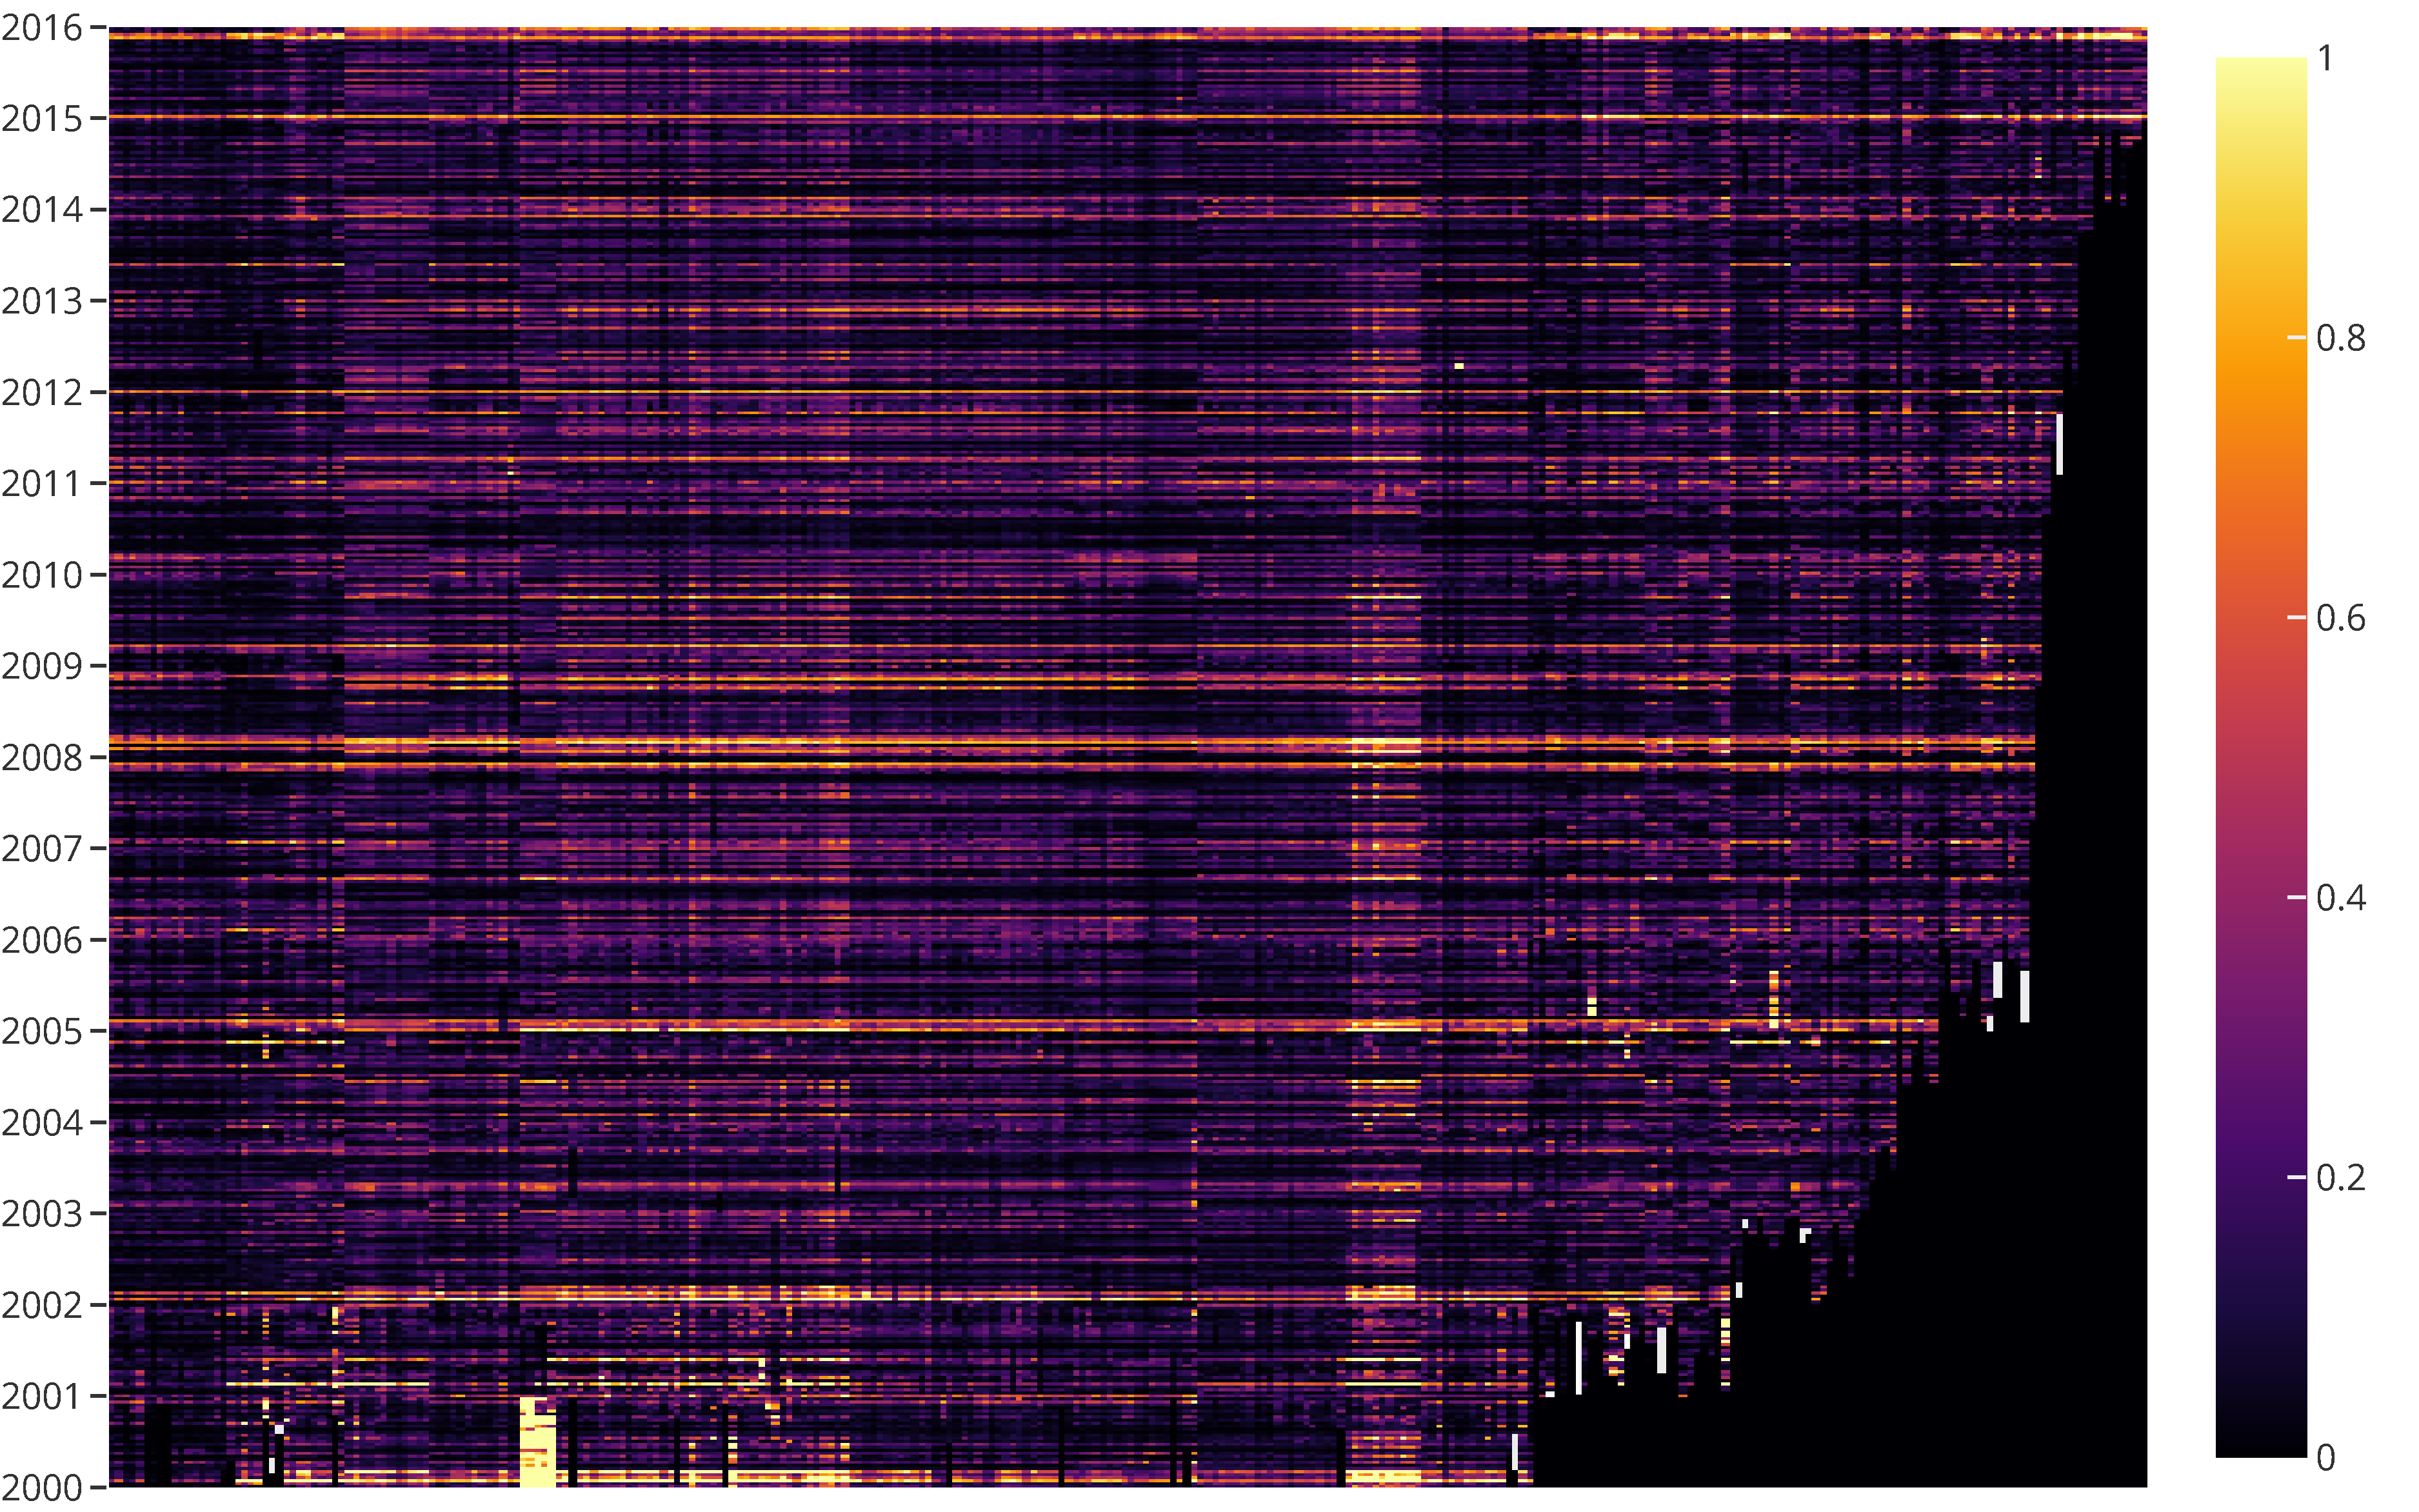
\includegraphics[width=0.75\textwidth]{data_availability_overall.pdf}
    }
    \\
    \subfloat[][CFs for the 33 modeled districts.]{
        \label{fig:availability_targets}
        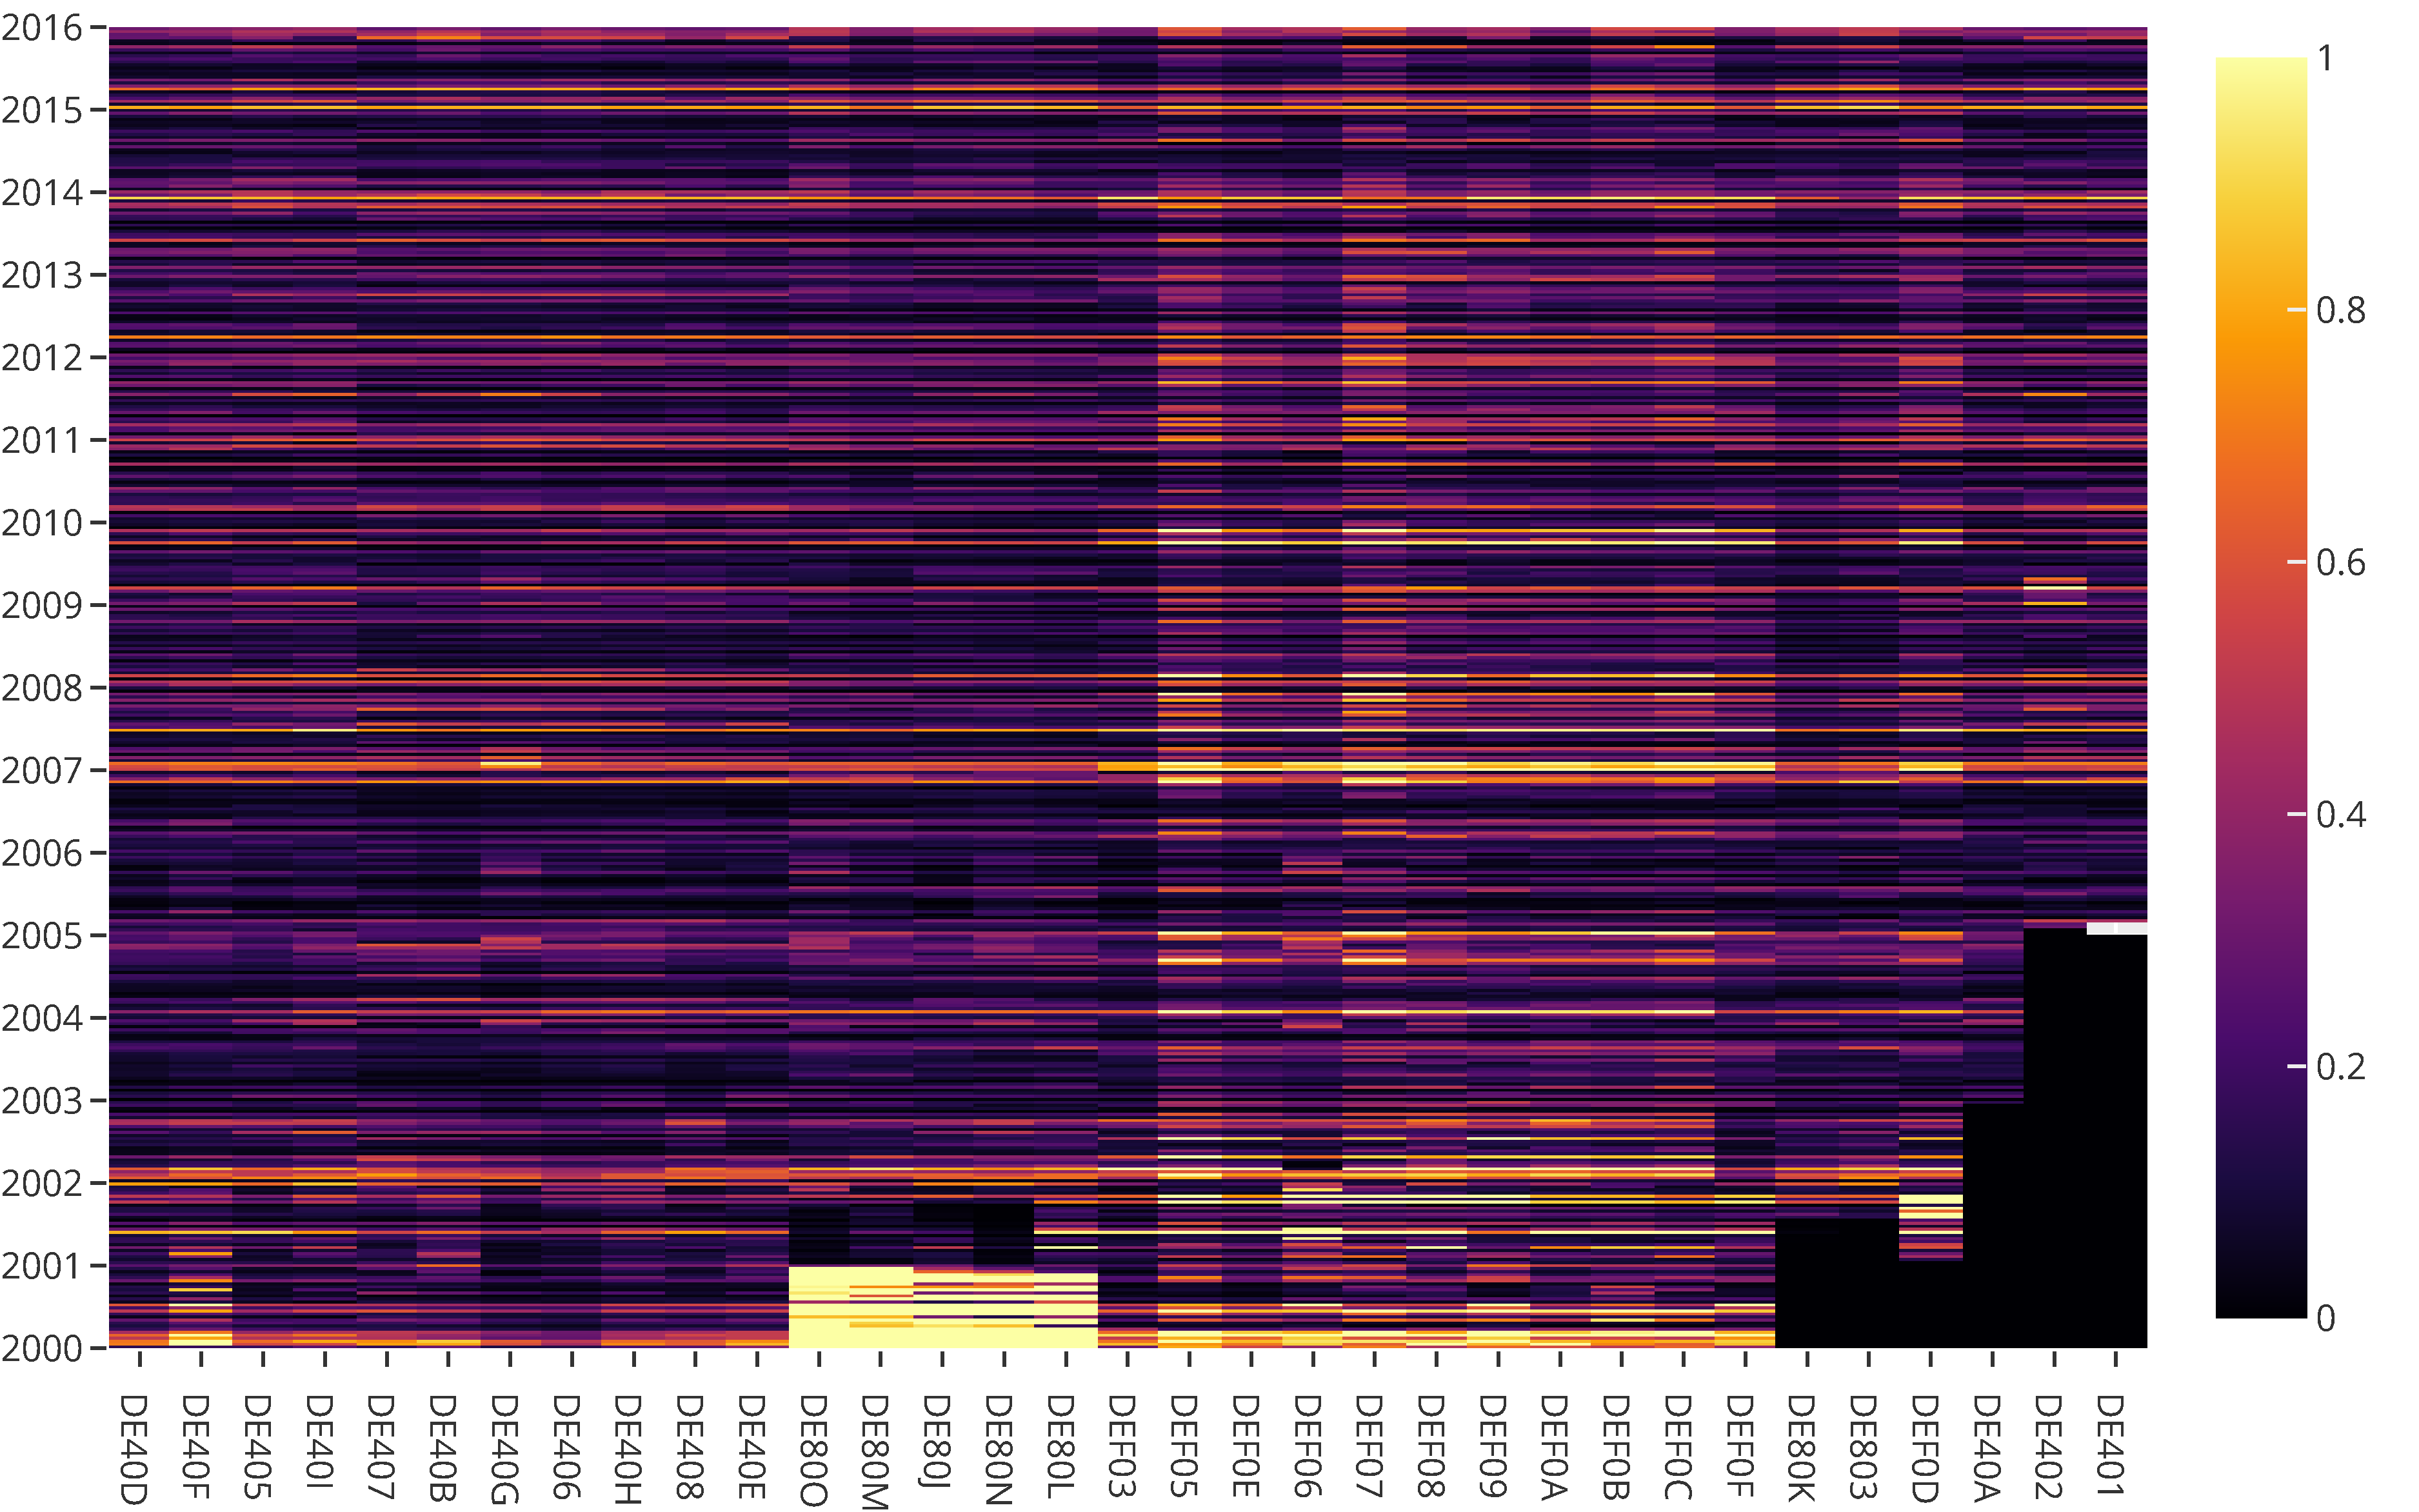
\includegraphics[width=0.75\textwidth]{data_availability_targets.pdf}
    }
\end{figure}

\begin{figure}[H]%
    \centering
    \caption{Spatio-temporal distribution of wind power generation capabilities.}
    \label{fig:germany_maps}
    \subfloat[][Turbines geodistribution.]{
        \label{fig:turbine_locations}
        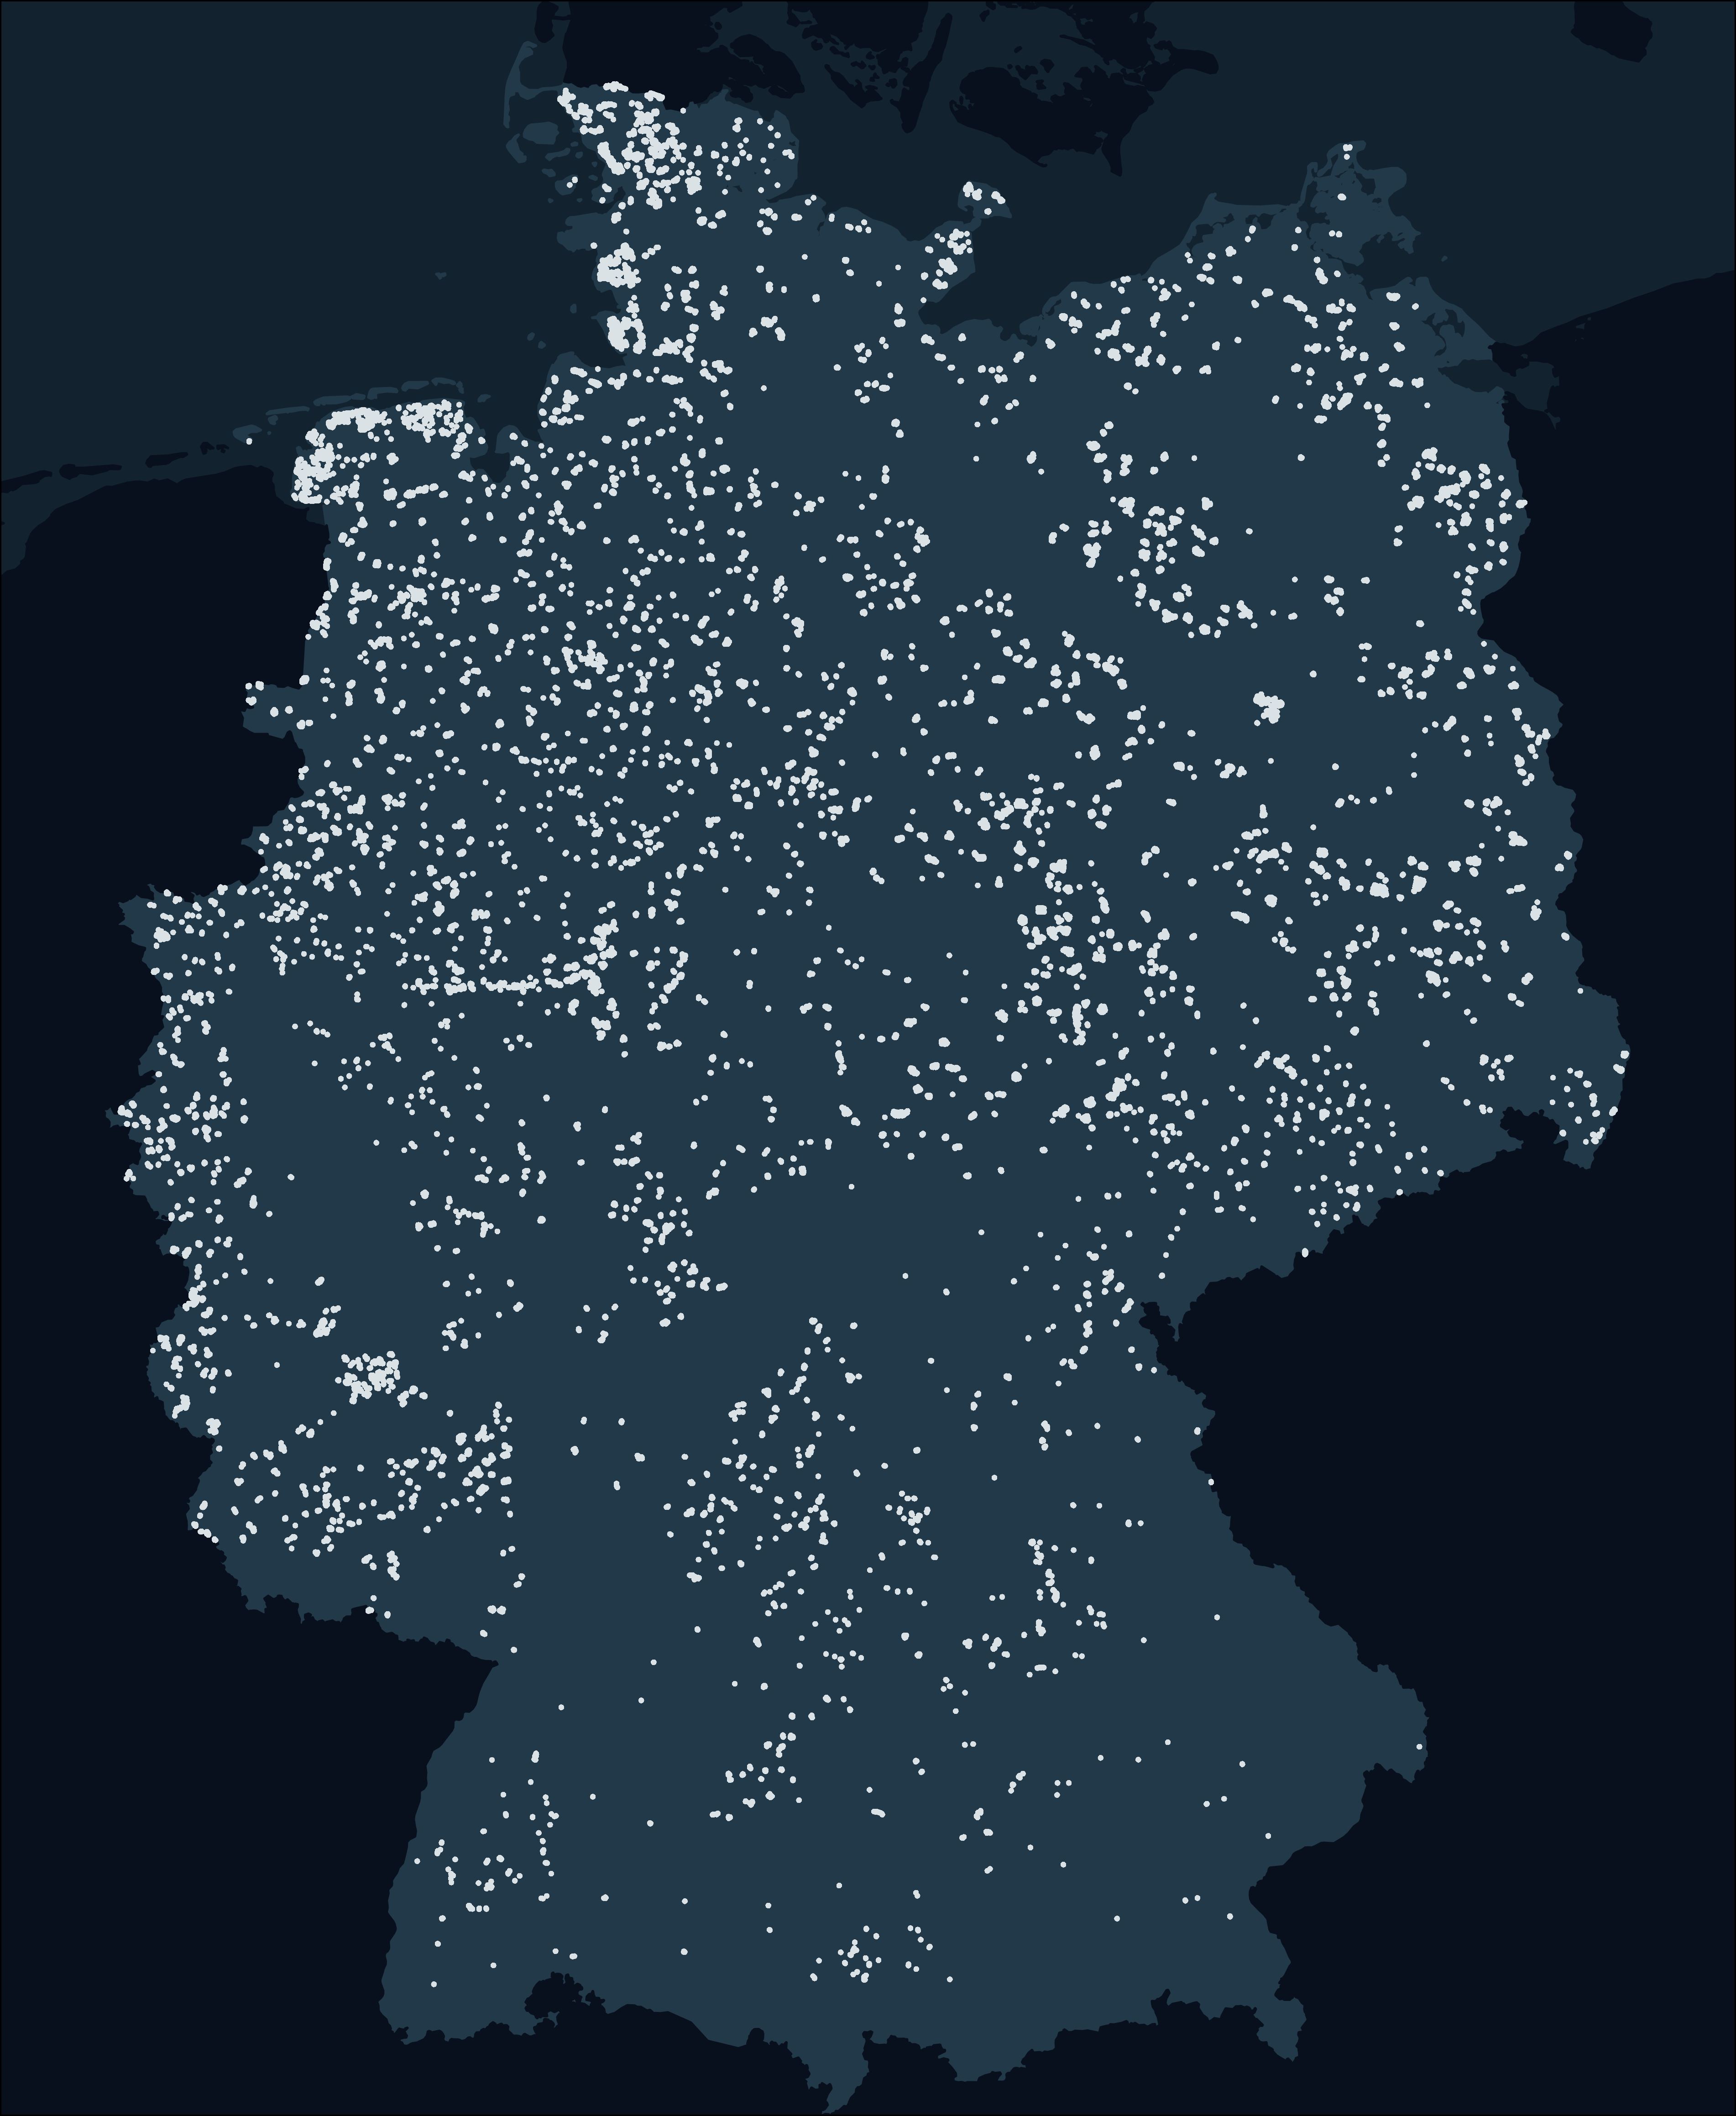
\includegraphics[width=0.5\textwidth]{turbines-spatial-distribution}
    }
    \subfloat[][Installed capacity by district.]{
        \label{fig:installed_capacity}
        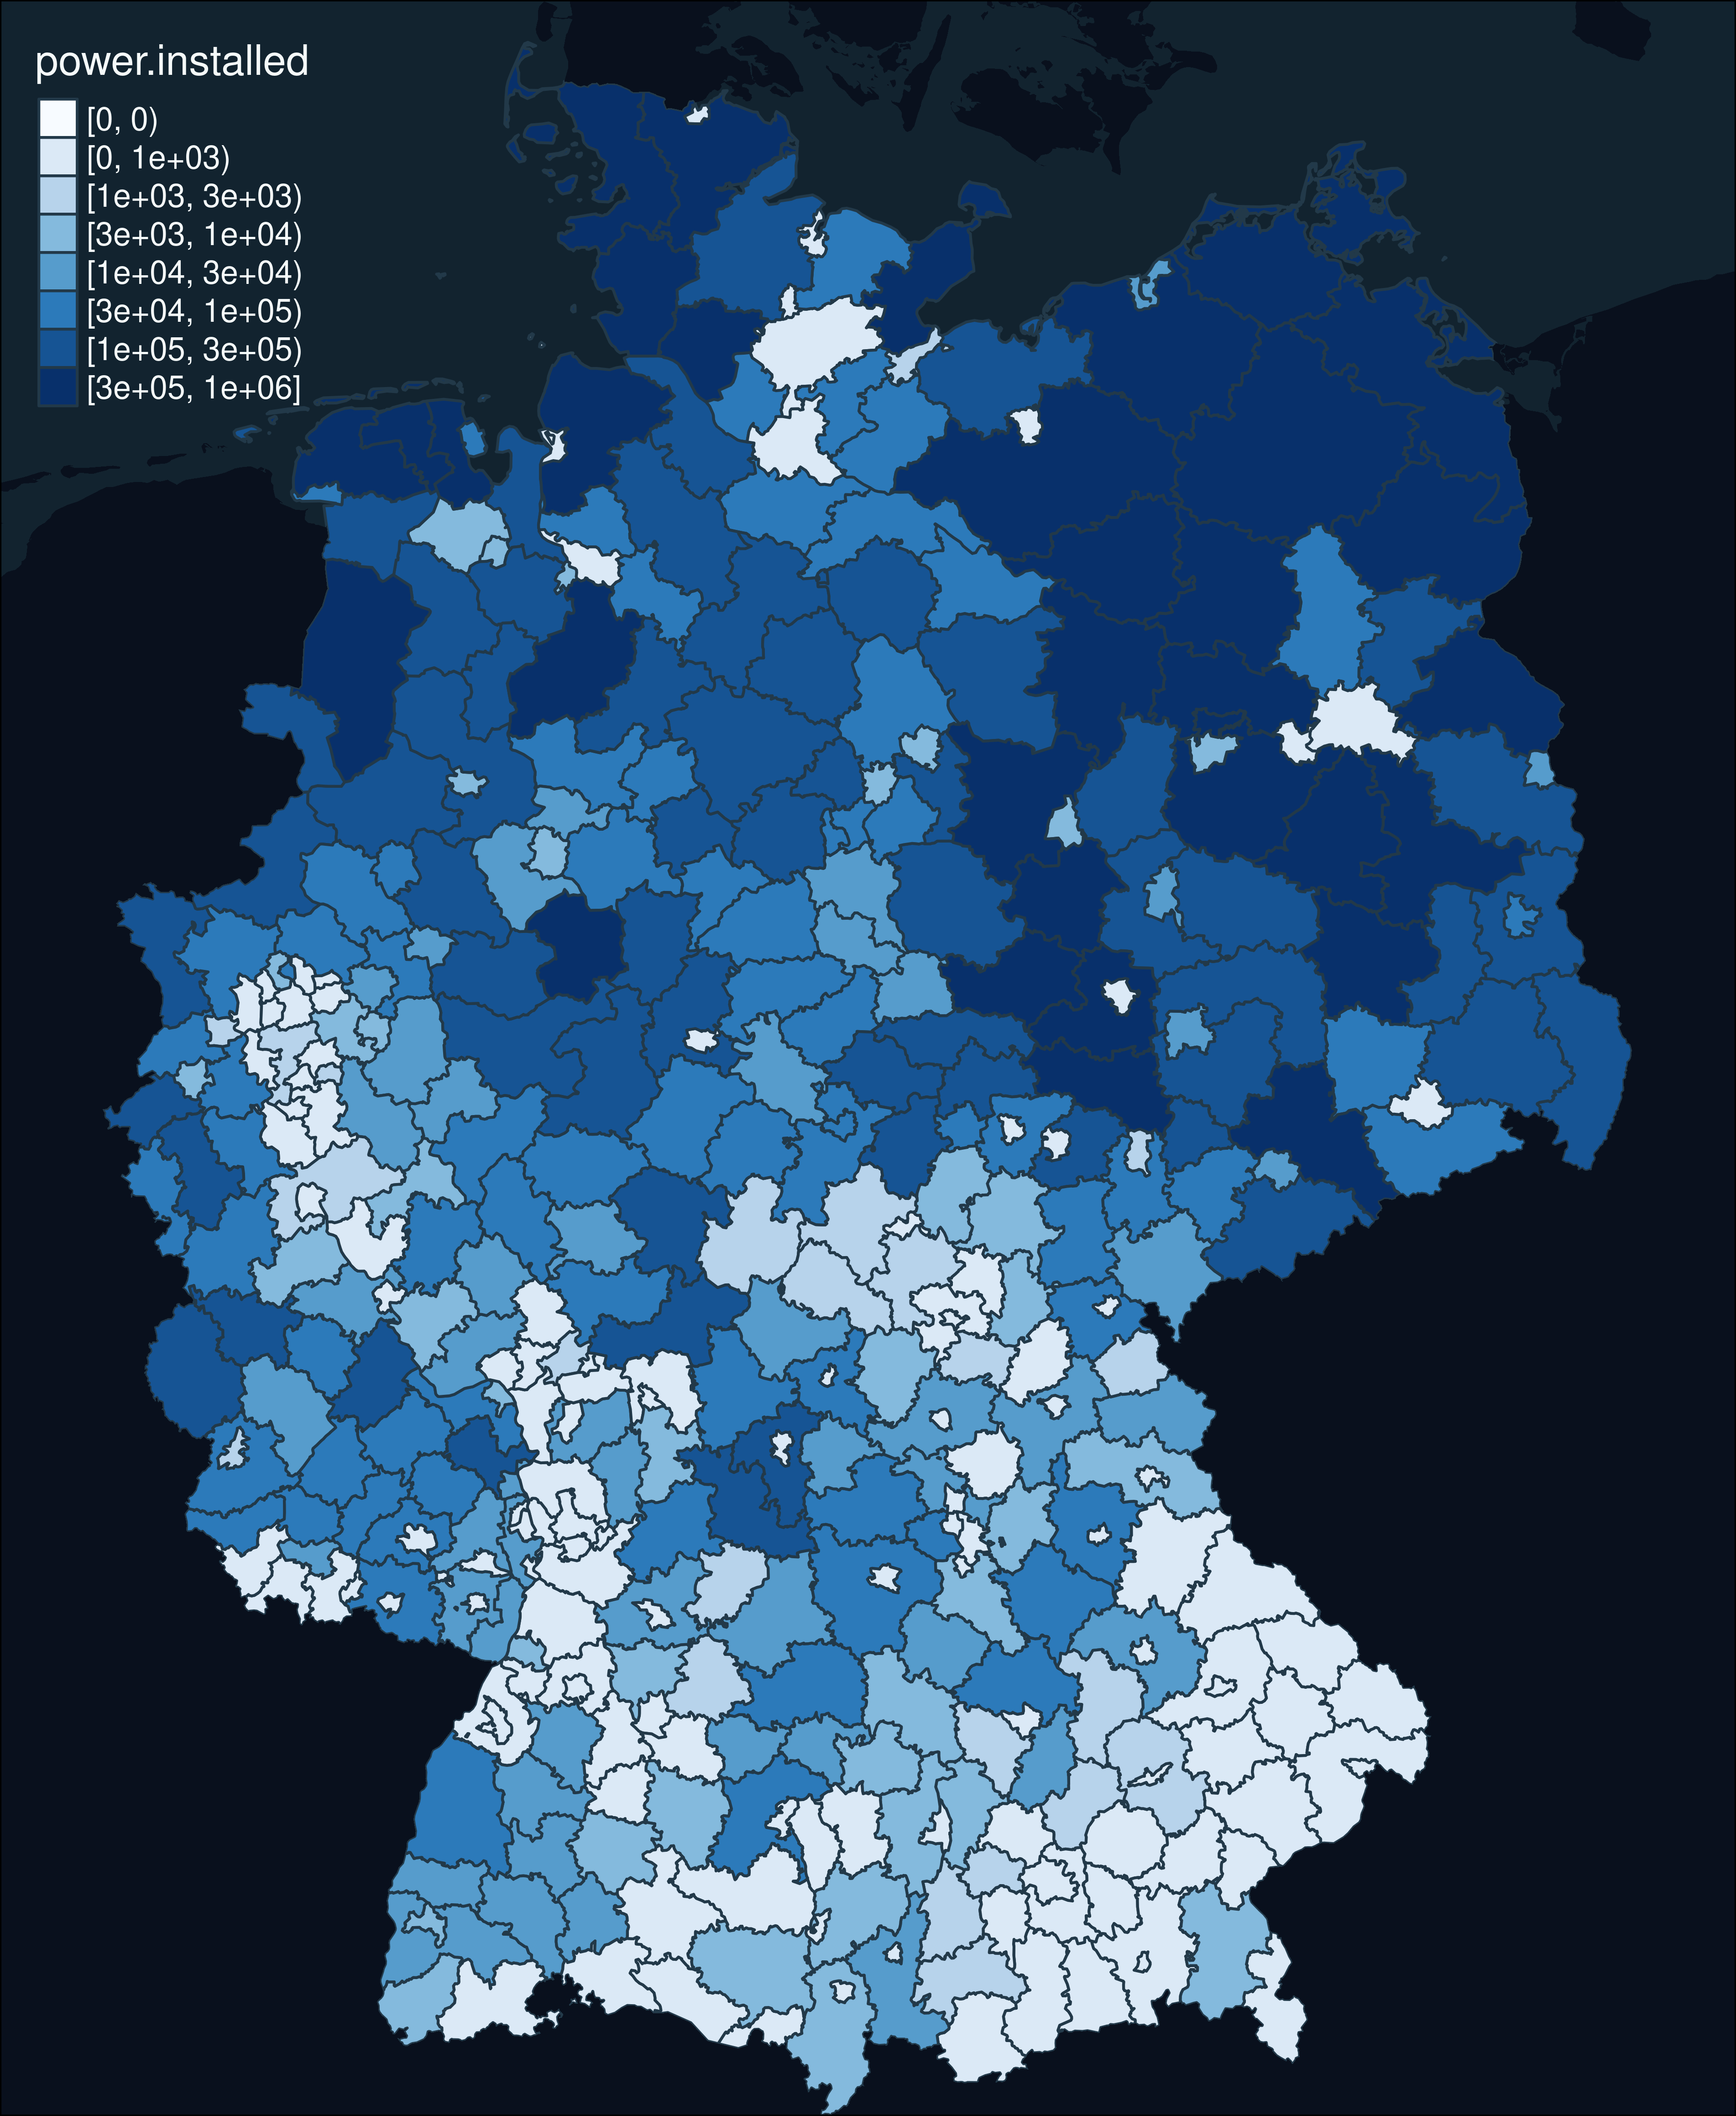
\includegraphics[width=0.5\textwidth]{power-installed-map}
    }
    \\
    \subfloat[][Geodistribution over time of rated power in new commissionings.]{
        \label{fig:spacetime_turbines}
        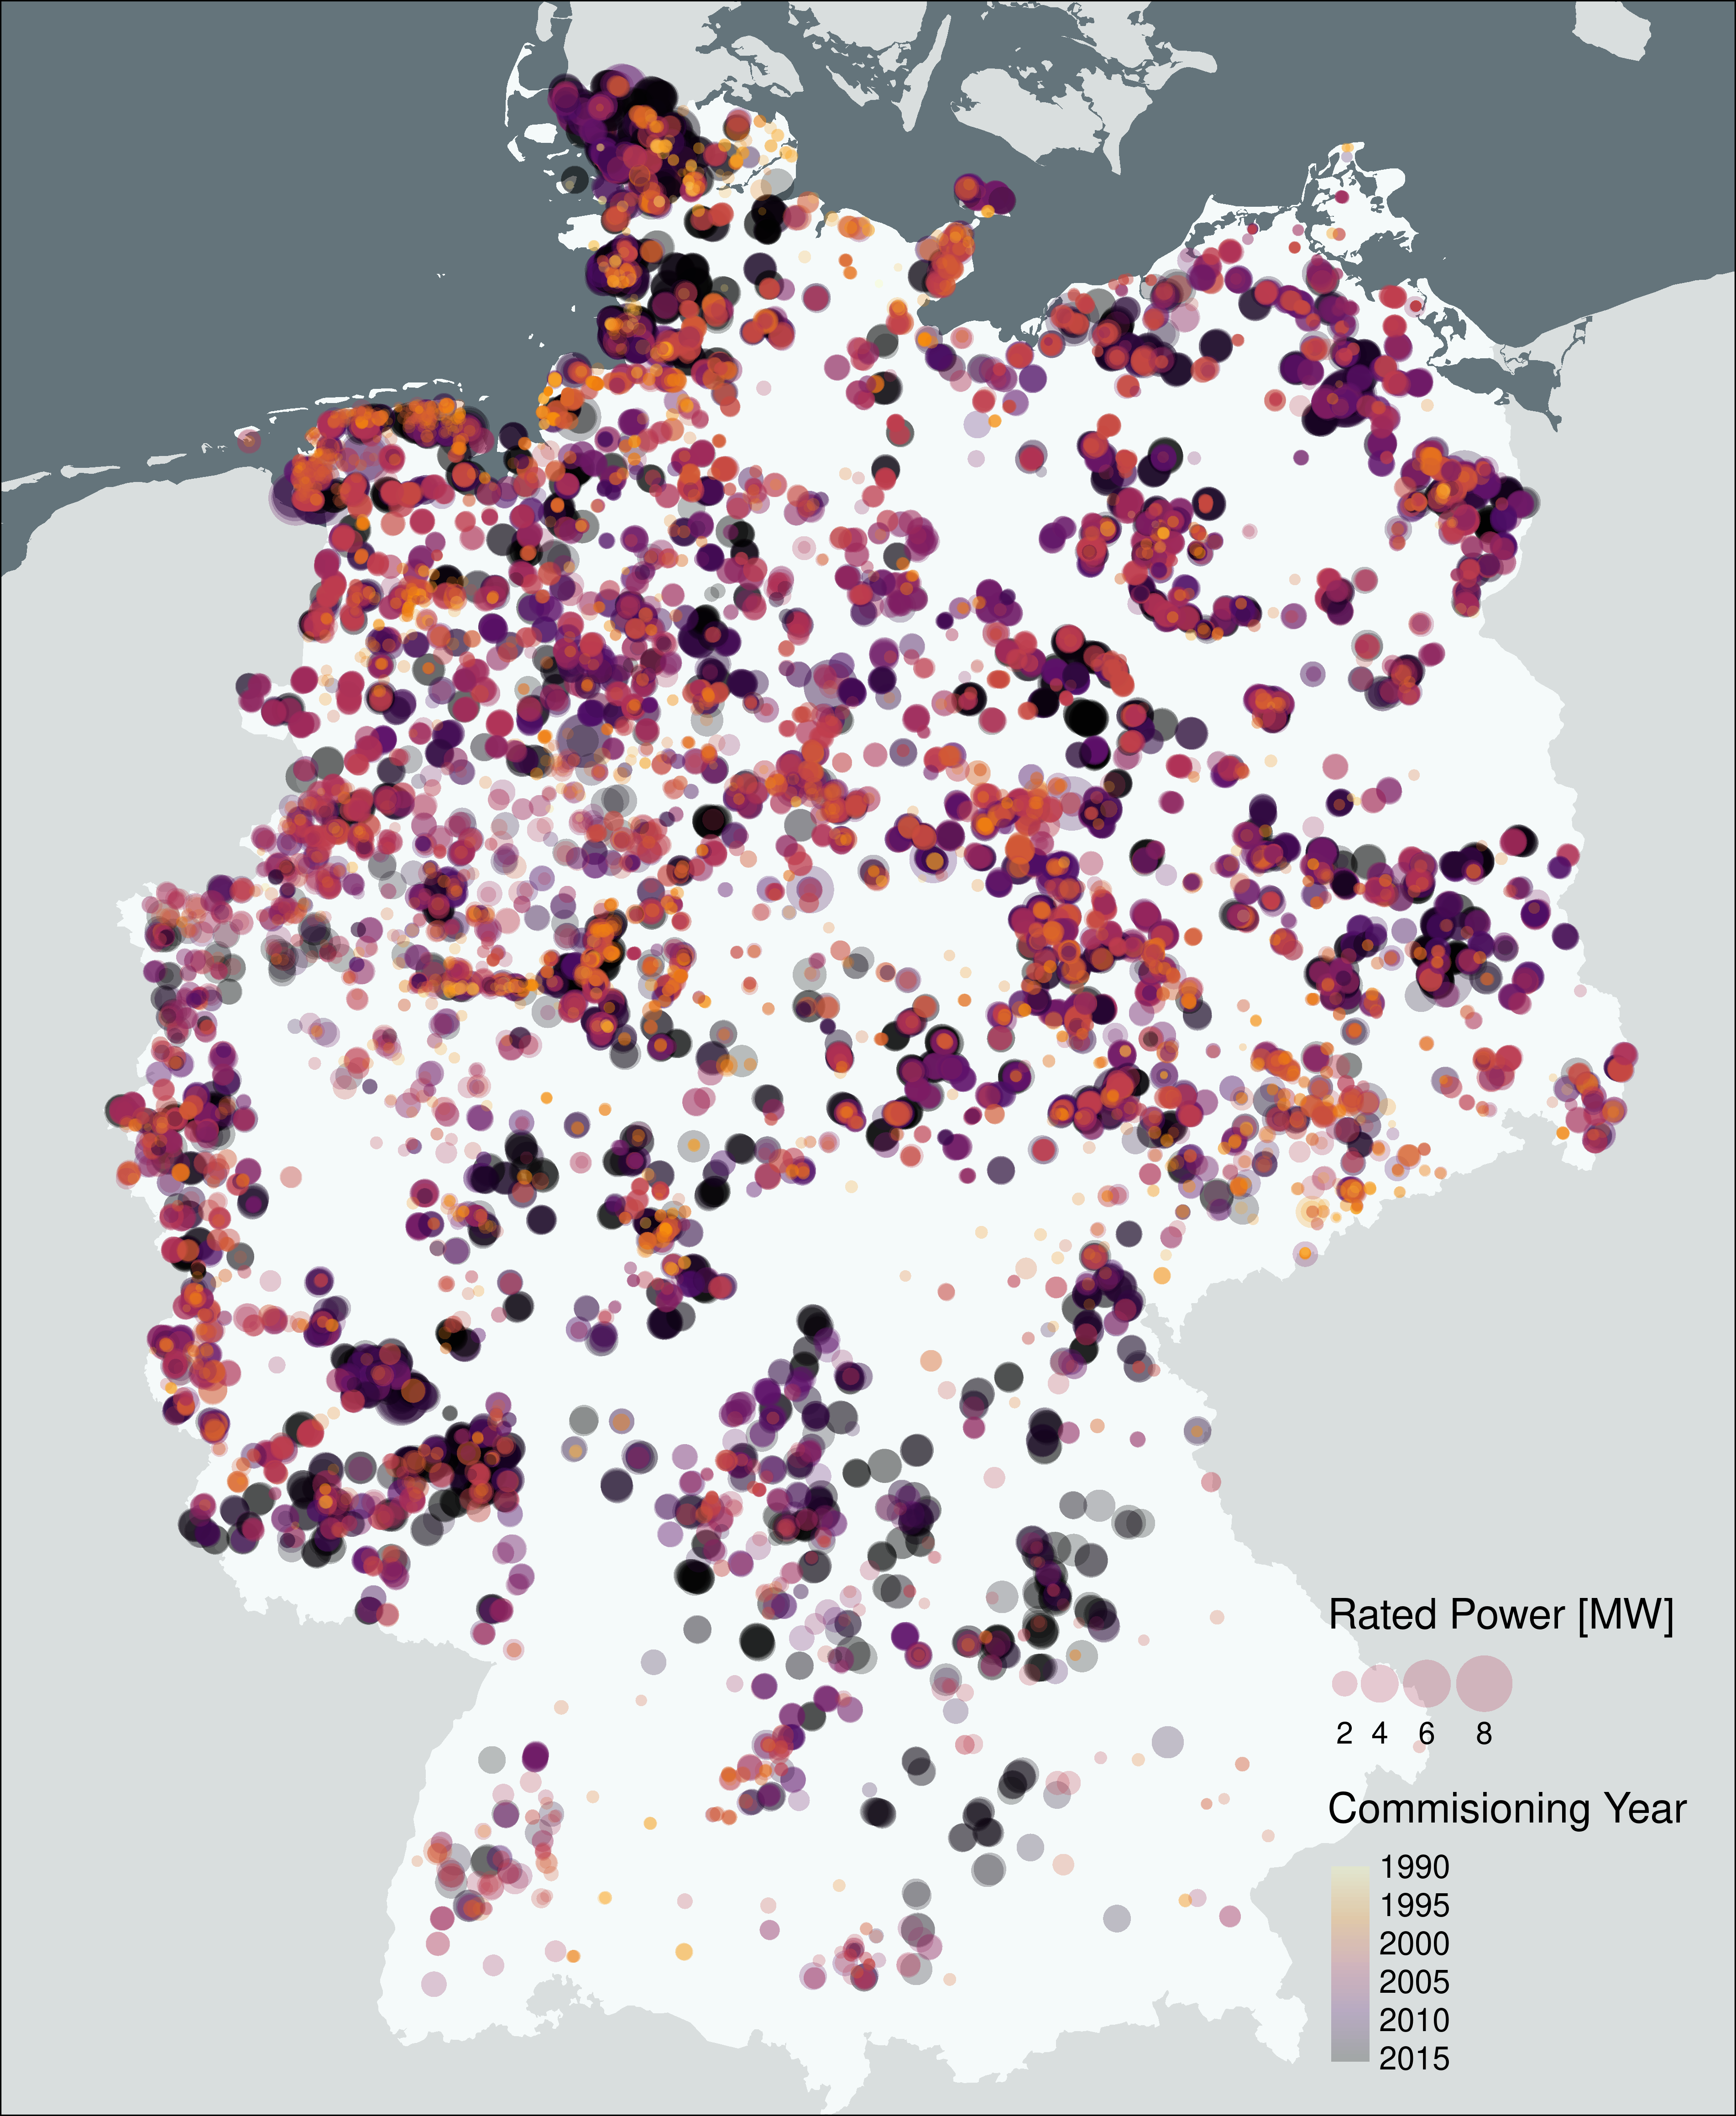
\includegraphics[width=0.75\textwidth]{map_turbines_locations_20200701_230854_fav}
    }
\end{figure}

The second step in our analysis concerned the determination of (1) how power generation is distributed and (2) what is a typical production behavior.
The kernel-estimated density function for the districtwise, yearly average power generation (e.g. figure \ref{fig:yearly_power_generation}) suggests a unimodal, approximately log-normal distribution.

\begin{figure}[H]%
	\centering
    \caption{Distribution of yearly districtwise wind power generation.}
    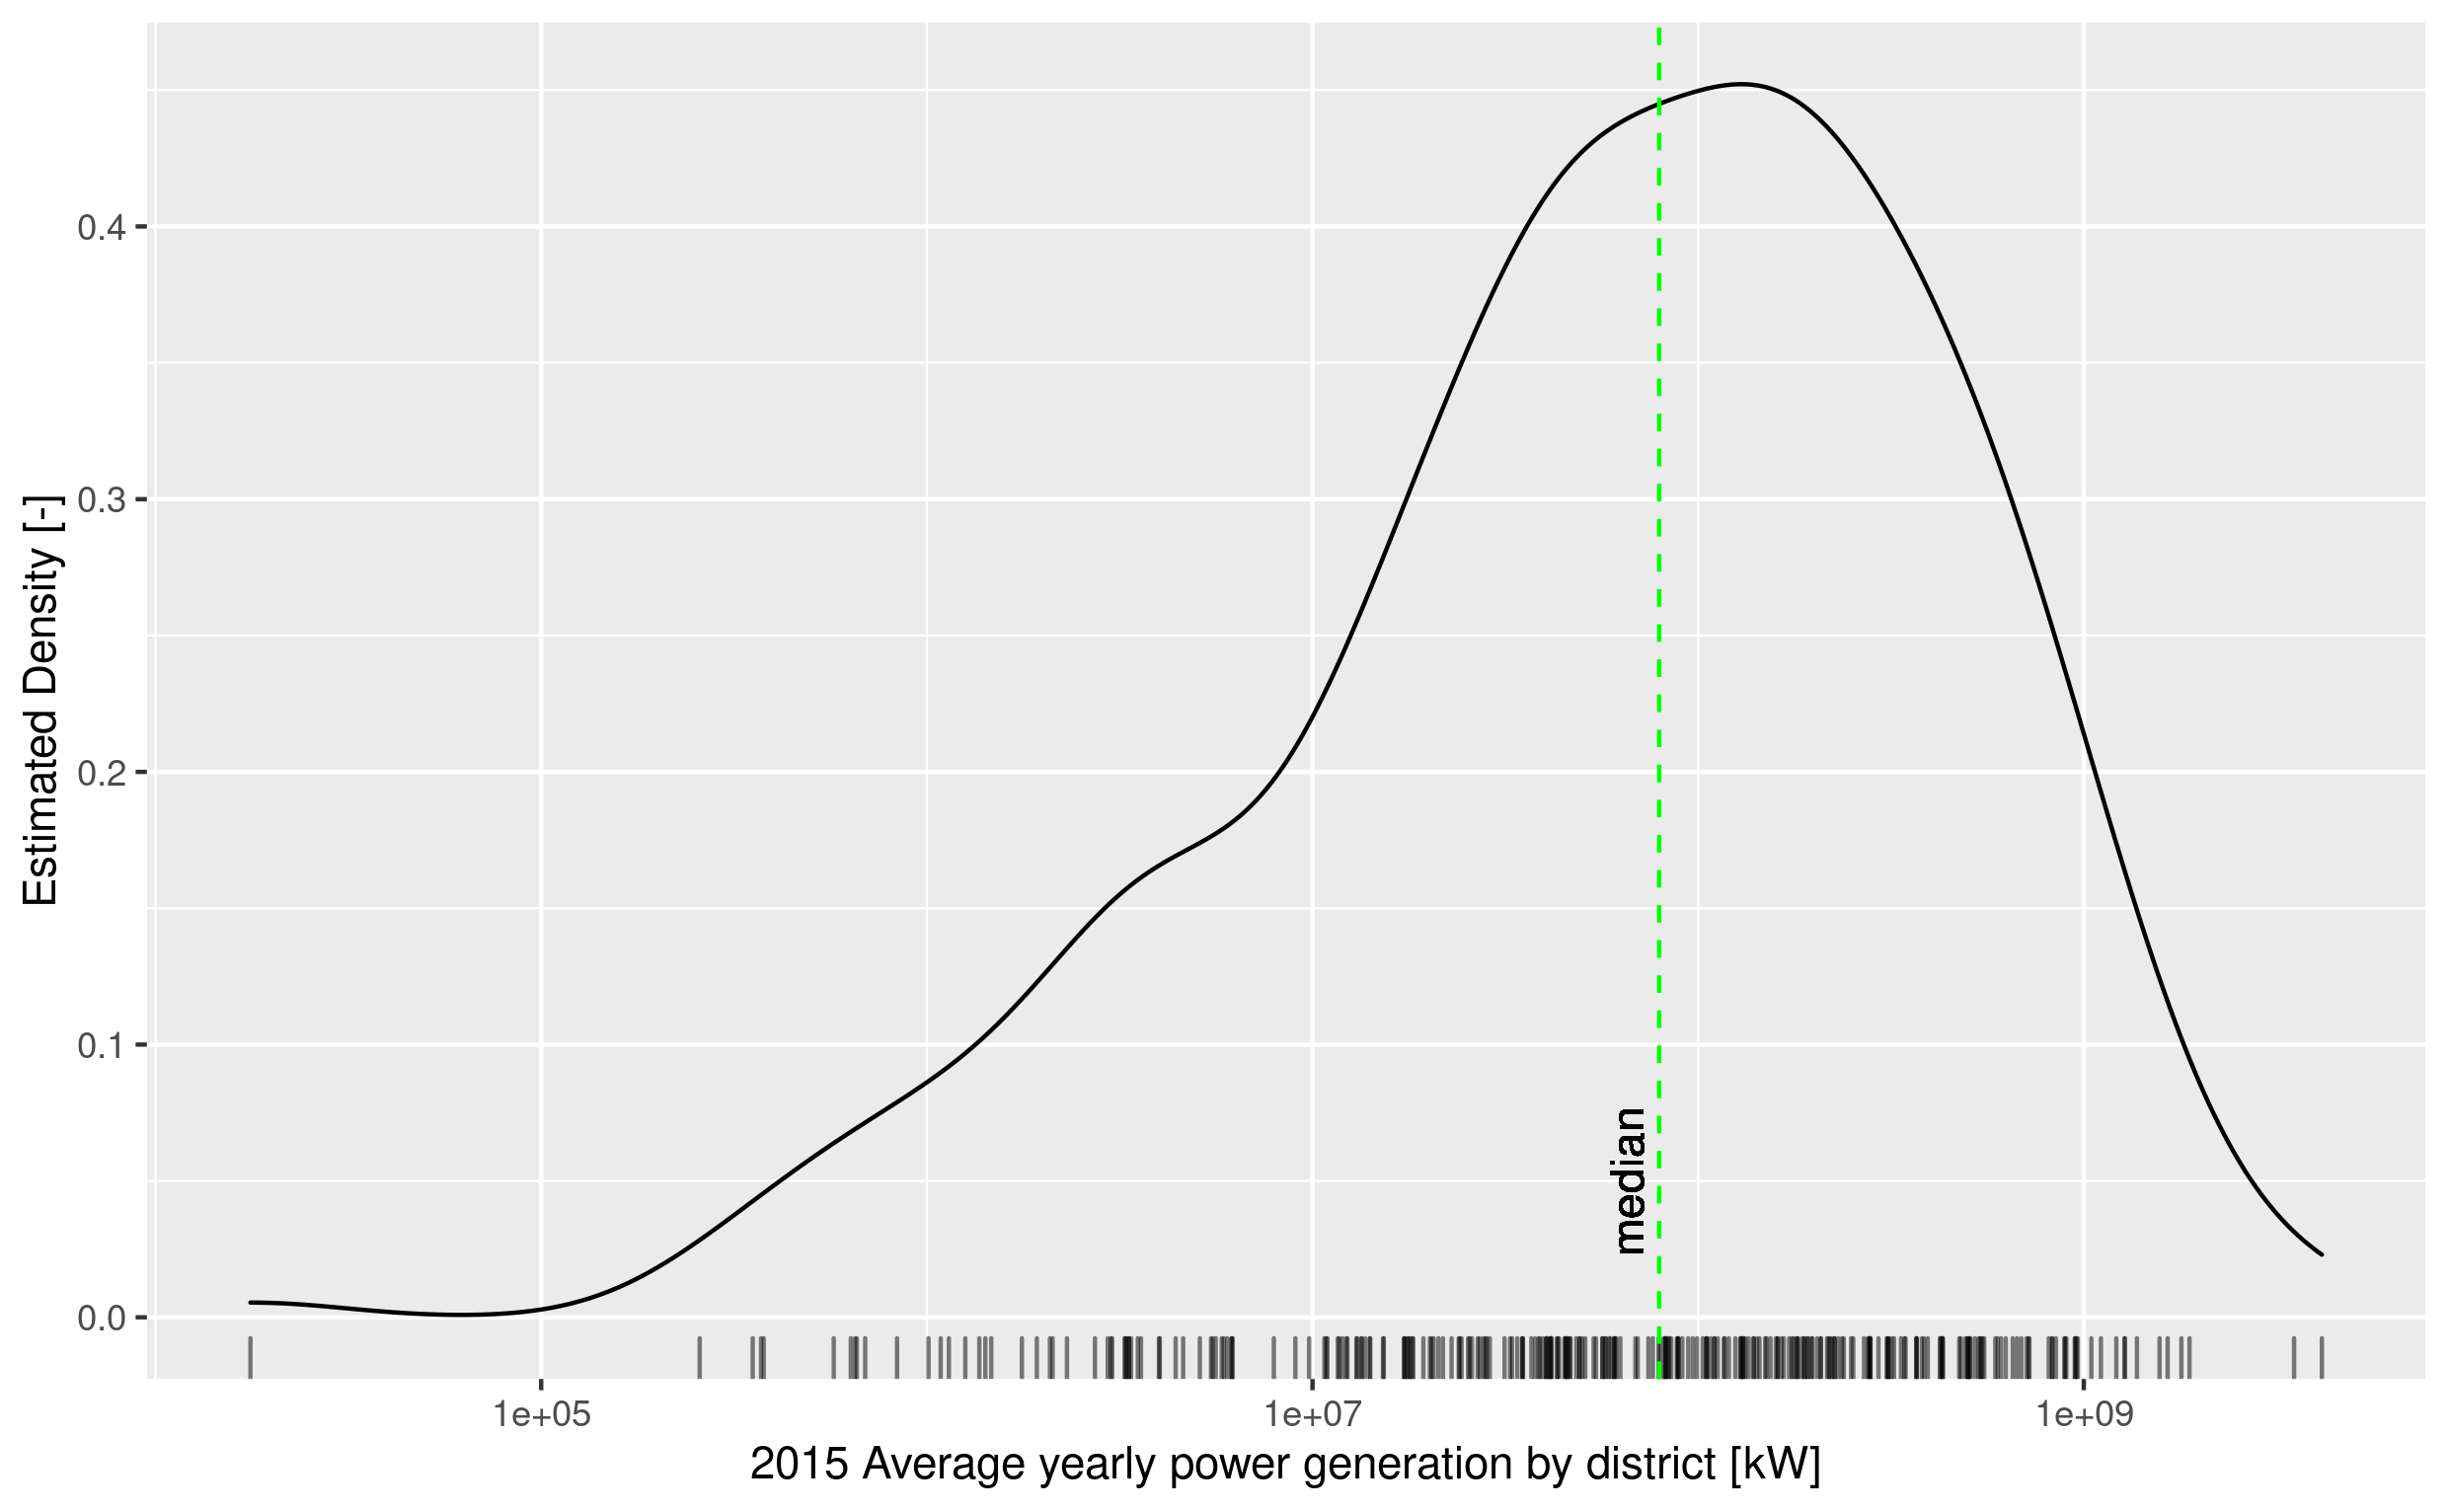
\includegraphics[width=0.8\textwidth]{power-generated-yearly-distribution}
	\label{fig:yearly_power_generation}
\end{figure}

We noticed near-median yearly power productions tend to be distributed across time as the one shown in figure \ref{fig:deb22_production_2015}.
The observed Weibull distribution is in agreement with accounts in the literature \cite{blaabjerg2017electronics, engeland2017variability, he2014short-term}.
Here, we notice an important behavior trend: not only the measurements values vary, but also their amplitude, as new turbines are commissioned (and decommissioned).
This is specially significant in the case of Germany, where wind power generation rapidly increases its share in the energy portfolio.

\begin{figure}[H]%
	\centering
    \caption{A typical power generation (in kW) in a year, as represented by the district of Bernkastel-Wittlich (DEB22).}
    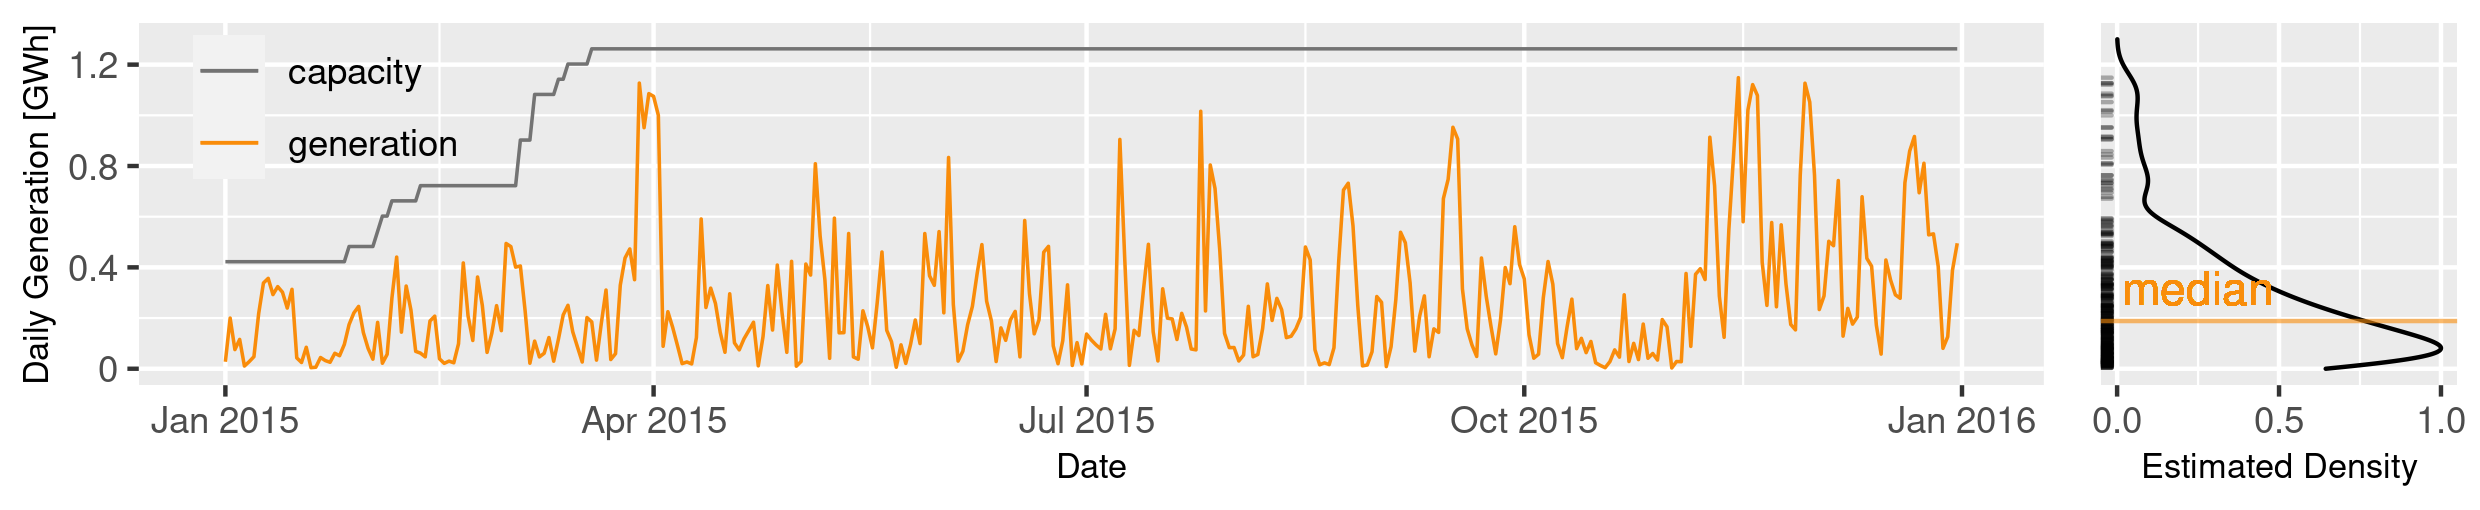
\includegraphics[width=\textwidth]{wpg-daily-typical-ts_20200701_155716_fav.png}
	\label{fig:deb22_production_2015}
\end{figure}

This might pose a significant limitation to models inferred from historic data for power generation alone, as they would be unable to capture the correlations arising from the causal effect of (de-)commissionings on future values of power generation.
In other words, trained on the dataset as it is, models would be unable to account for eventual sudden increases in power generation due to new commissionings, eventually incurring in drastically underestimating forecasts.
Furthermore, we would expect this effect to be more pronounced for longer forecast horizons, as the probability of new commissionings for the forecast period would increase.

One way to address this would be to provide to the models an exogenous feature which informed it about new commissioning ahead.
Not every forecasting approach supports this, however, as in the case of historical average or single-input ARIMA variants.
This would thus limit the comparability of methods performance.

For this reason, we use another approach in this work.
Essentially, we train the models to predict a normalized version of the time series and handle the effect by re-scaling model outputs in a model-agnostic, post-processing step.
More specifically, we scale each time series value by the installed capacity for the specific district and point in time.
In the renewables field, the resulting scaled variable is known as the Capacity Factor ($CF$).
The resulting time series are illustrated in figures \ref{fig:deb22_production_2015_cf} and \ref{fig:all_cf}.

\begin{figure}[H]%
	\centering
    \caption{A typical power generation (in Capacity Factor) in a year, as represented by the district of Bernkastel-Wittlich (DEB22).}
    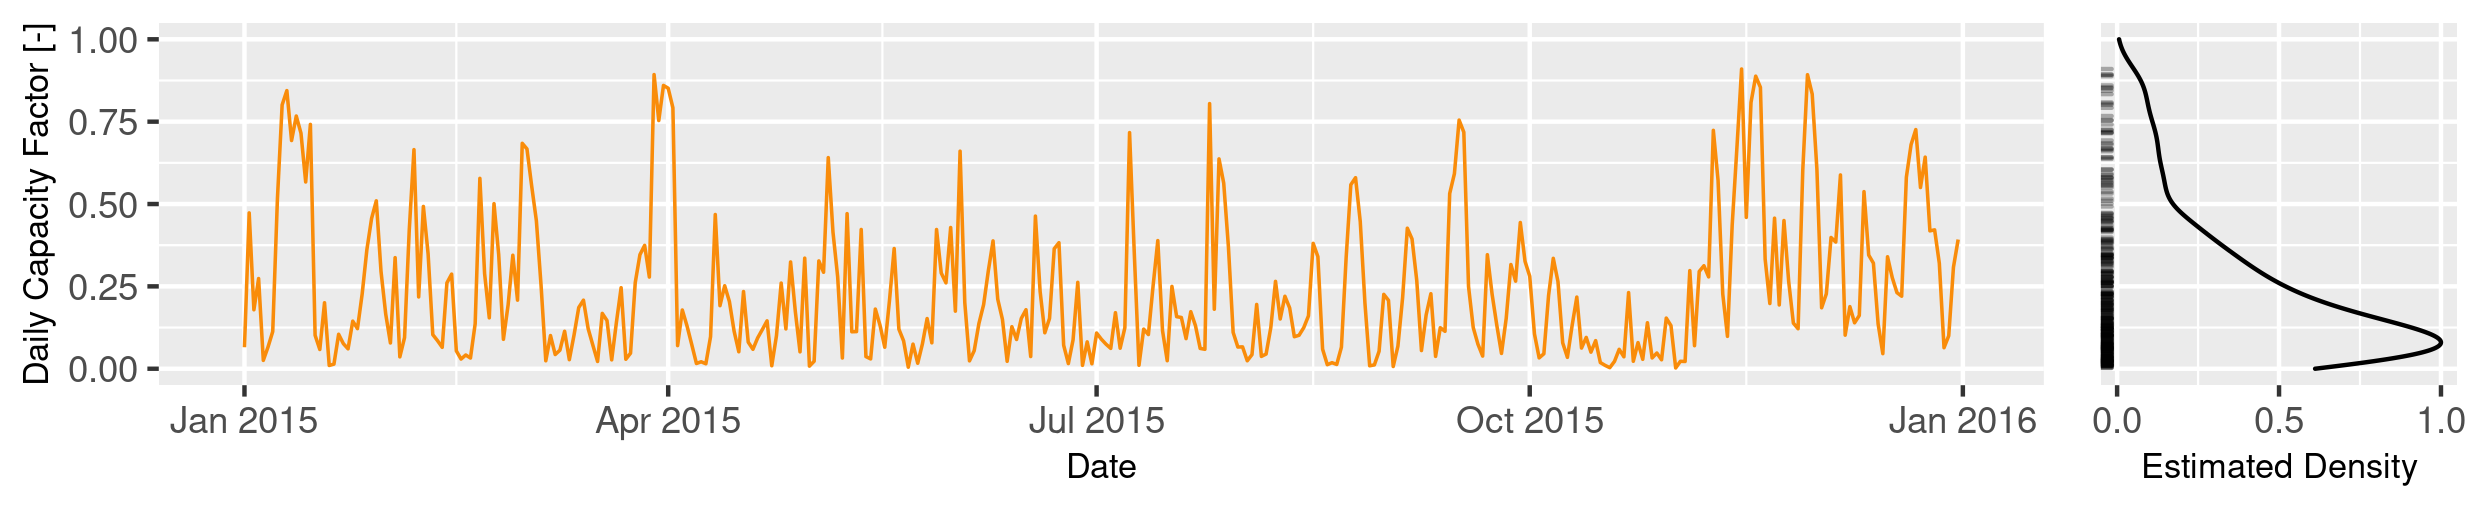
\includegraphics[width=\textwidth]{wpg-cf-daily-typical-ts_20200703_075319}
	\label{fig:deb22_production_2015_cf}
\end{figure}

\begin{figure}[H]%
	\centering
    \caption{Power generation in terms of CF for all districts. The highlighted CF curve refers to Bernkastel-Wittlich (DEB22).}
    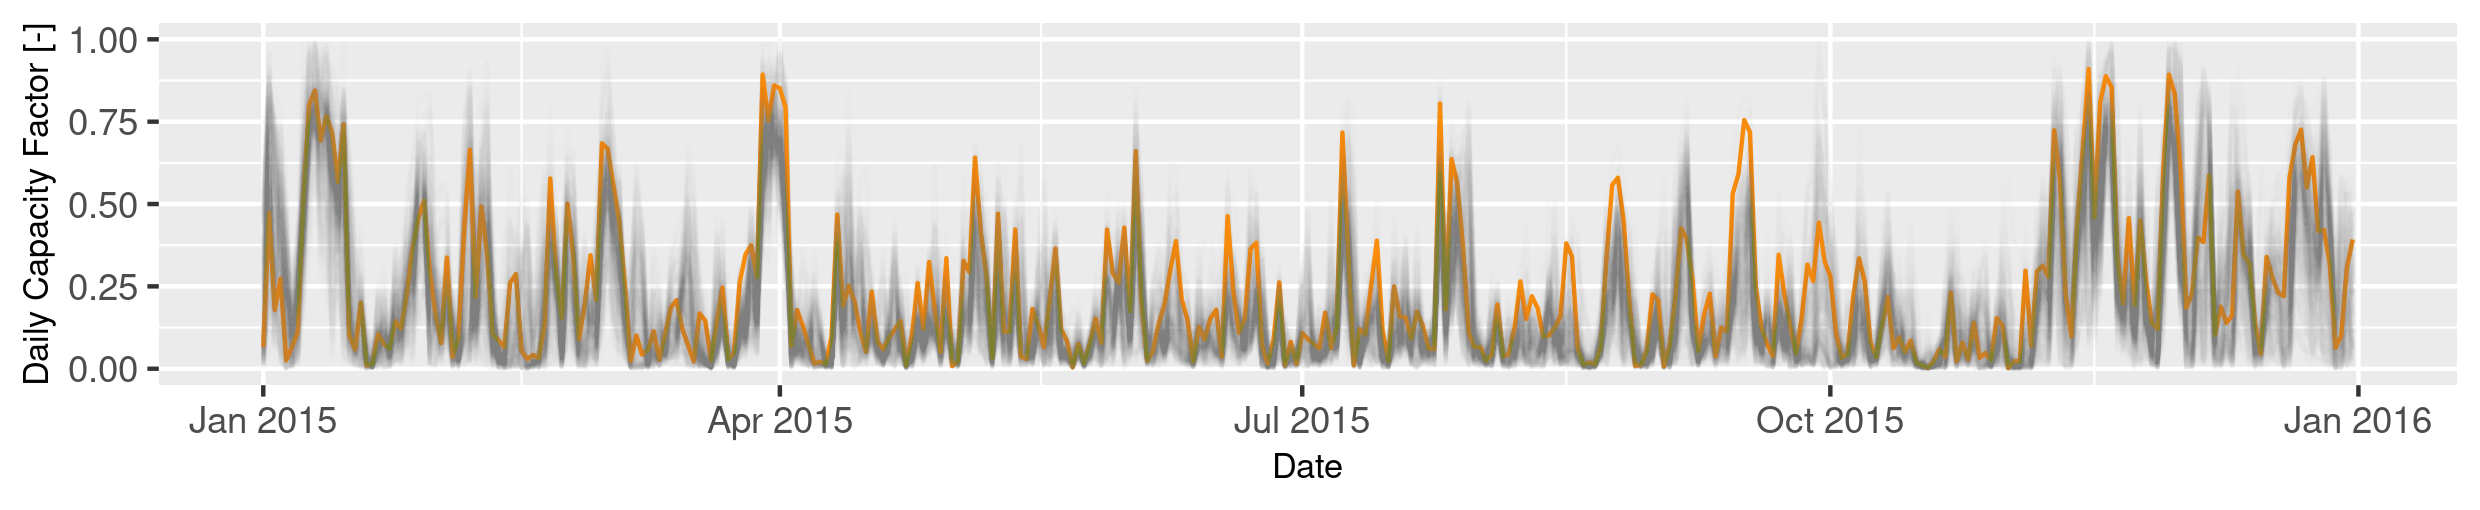
\includegraphics[width=\textwidth]{wpg-cf-daily-all-ts_20200701_163815_fav}
	\label{fig:all_cf}
\end{figure}

While the transformation of time series from kW into Capacity Factors solves the issue concerning new commissionings, another issue involving the distribution of time series values remains.
Being Weibull-distributed, values in a time series would be concentrated around the median, thus less discernible from one another than if they were normally distributed, for instance.
Thus, we expect gains in terms of informational entropy and thus in model training cost and performance by properly scaling the model inputs.
The nature of the Weibull density function suggests that any linear scale such as the min-max scaling would not suffice to improve discernibility (informational entropy) in our data.
%As a consequence, the models performance would be unnecessarily more conditioned on the numerical precision, %which could eventually provoke unwanted loss of informational entropy.
%In fact, any linear transformation would incur in the same shortcoming.

In a third step of our exploratory data analysis, we investigated to what extent power generation is correlated in space and time.
For the spatial dependency, we inquired \textit{"how more similarly do closer districts behave than distant ones?"}.
We performed this by assessing how pairwise Spearman correlations between districts change as districts are more distant from one another \cite{engeland2017variability}.
We verified that pairwise Spearman correlations between closer districts are significantly higher than distant ones, evidencing a significant spatial character for power production (\ref{fig:correlogram}).
In fact, districts present significant correlations ($\rho_s>0.8$) for distances up to about 150 km.
This \textit{decorrelation distance} is in agreement with values found for Central Europe by other authors \cite{engeland2017variability}.

\begin{figure}[H]%
	\centering
    \caption{Spearman Correlations for all $nCR(296, 2)$ pairs of districts power generation (in CF) time series.}
    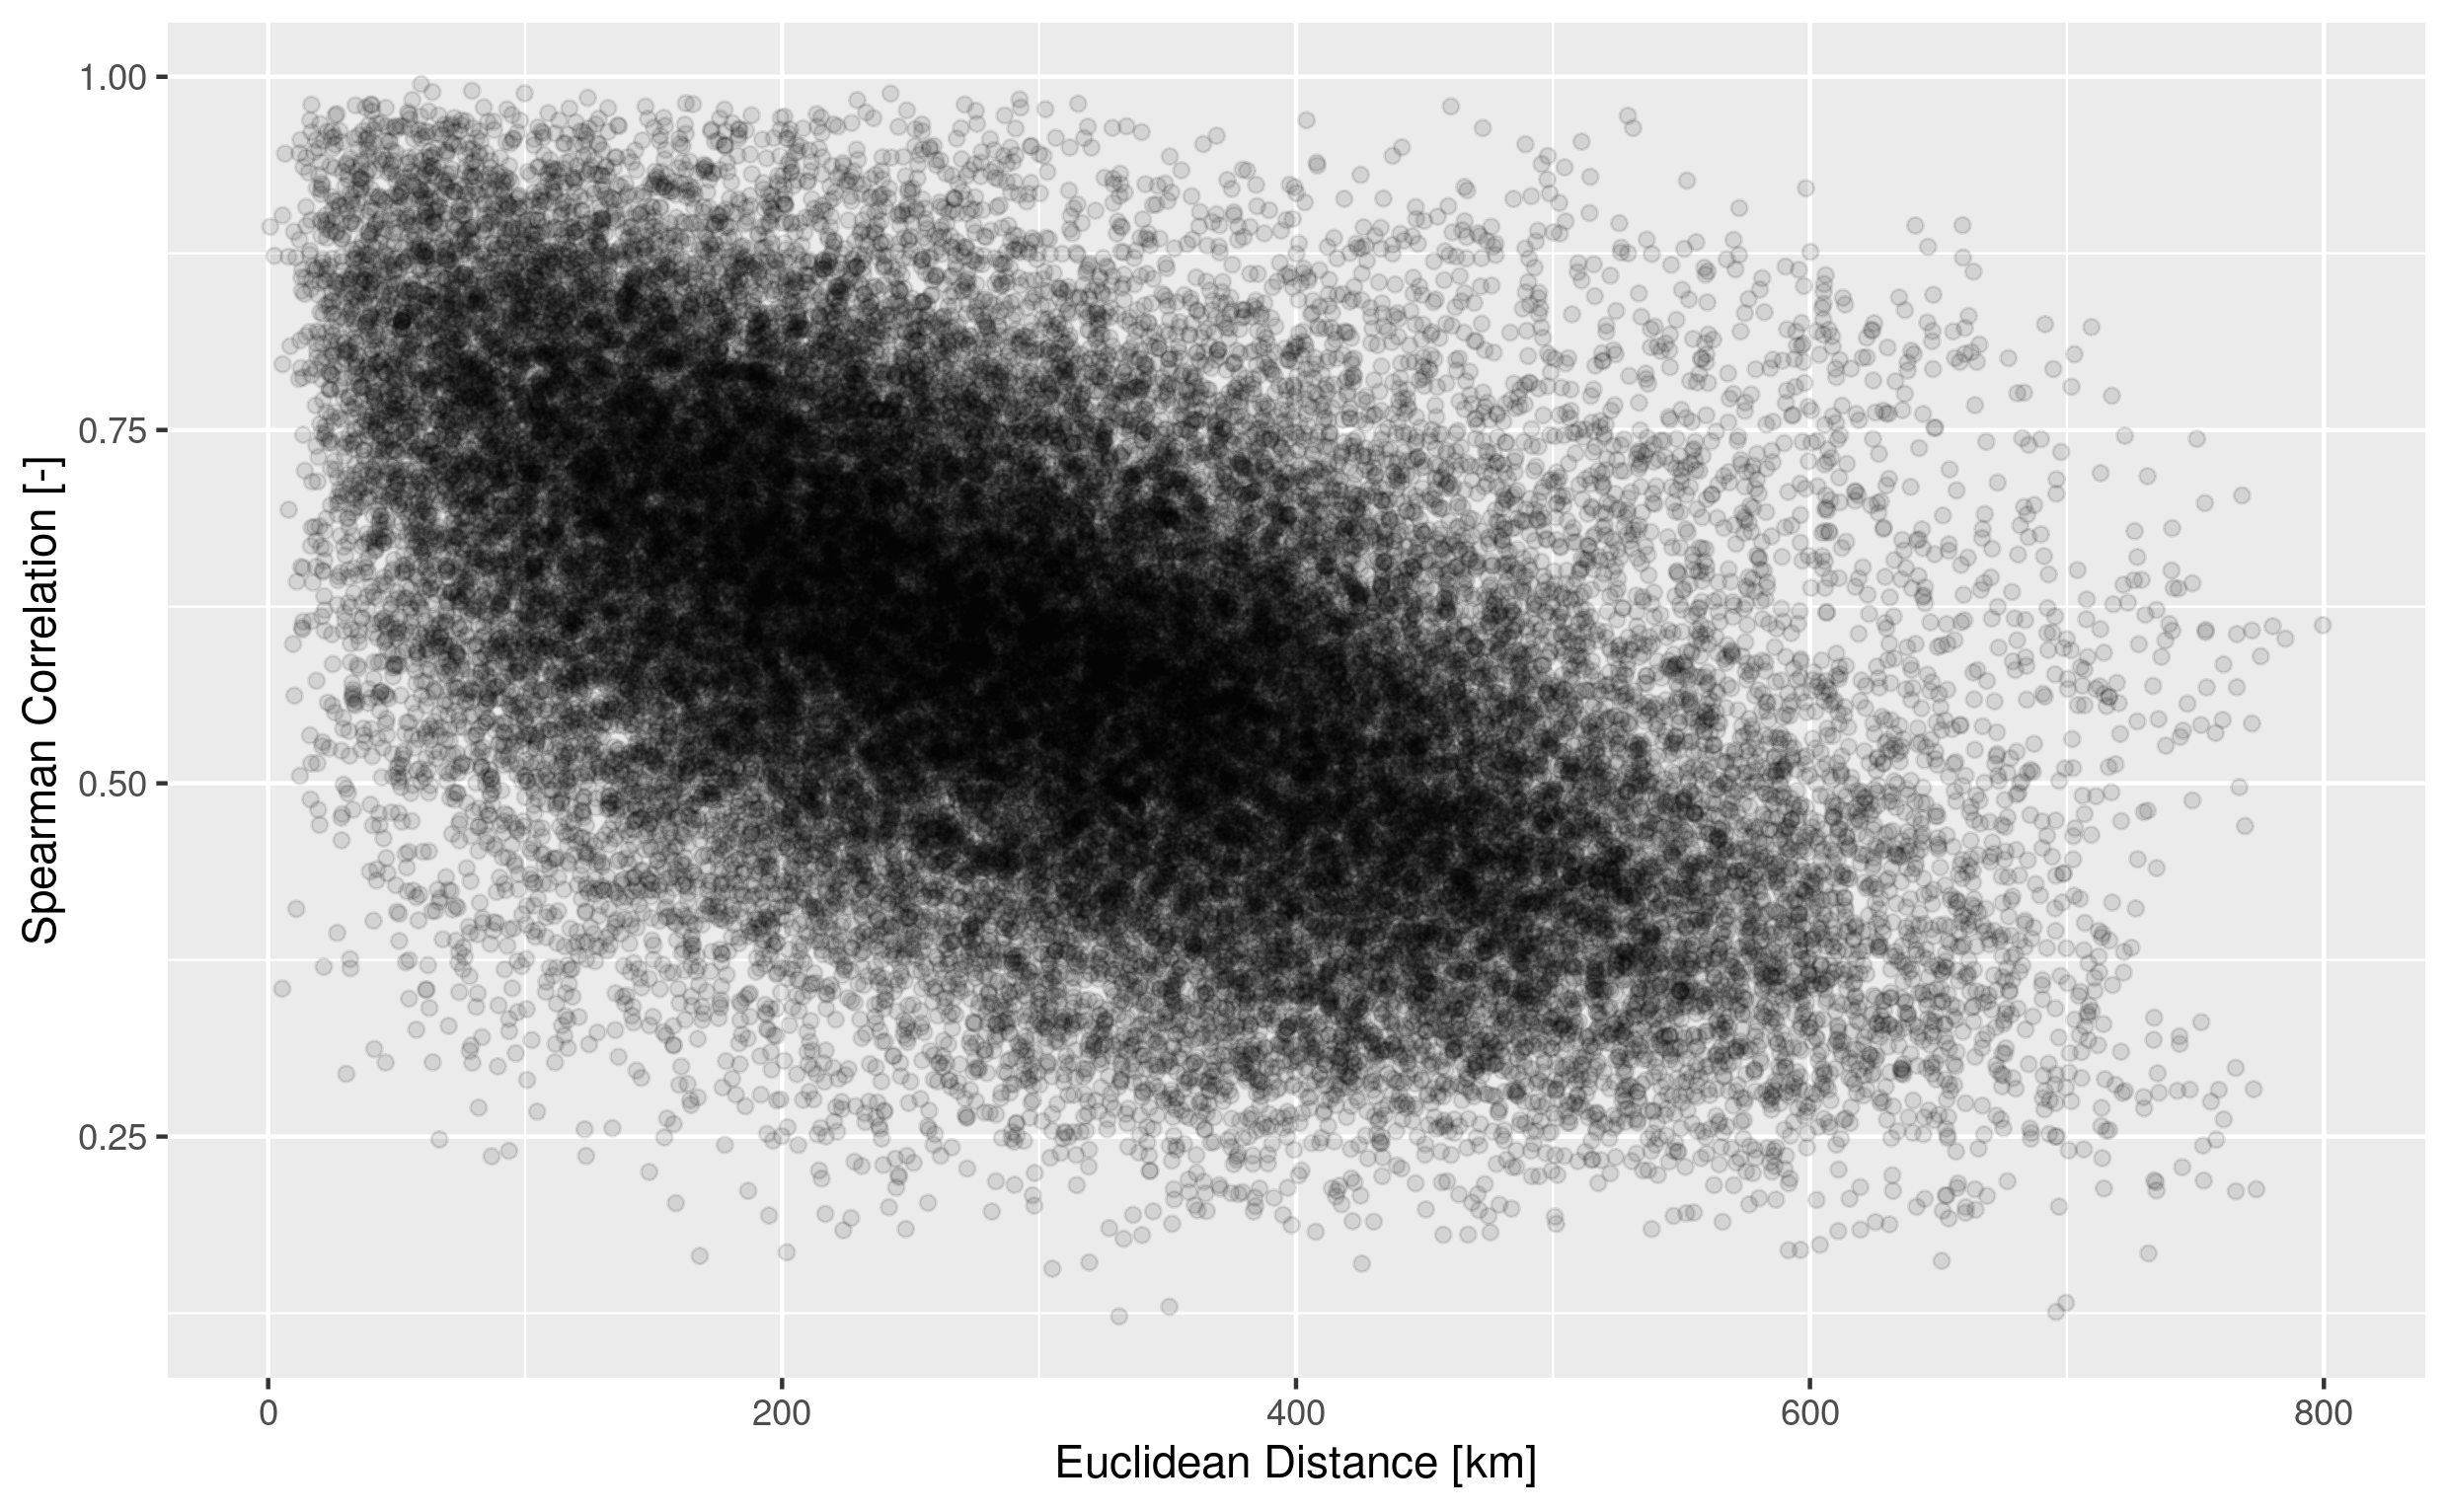
\includegraphics[width=0.8\textwidth]{correlation-spearman-vs-distance}
	\label{fig:correlogram}
\end{figure}

We followed a similar procedure to assess the temporal correlation between time series.
In order to attain evidence for this, we used cross-correlograms, which evaluate a cross-correlation function such as the Pearson coefficient $\rho$ as one time series is shifted in time in relation to the other time series.
Figure \ref{fig:ccf} shows an instance of correlogram for a pair of districts at decorrelation distance.
Figure \ref{fig:ccf_all} presents the superposition of all correlograms.
We verify a decorrelation time delay of 12 hours, which is in agreement with the literature for Central Europe \cite{engeland2017variability}.

\begin{figure}[H]%
	\centering
    \caption{Cross-correlogram for the districts sample pair (DEB22, DEE145).}
    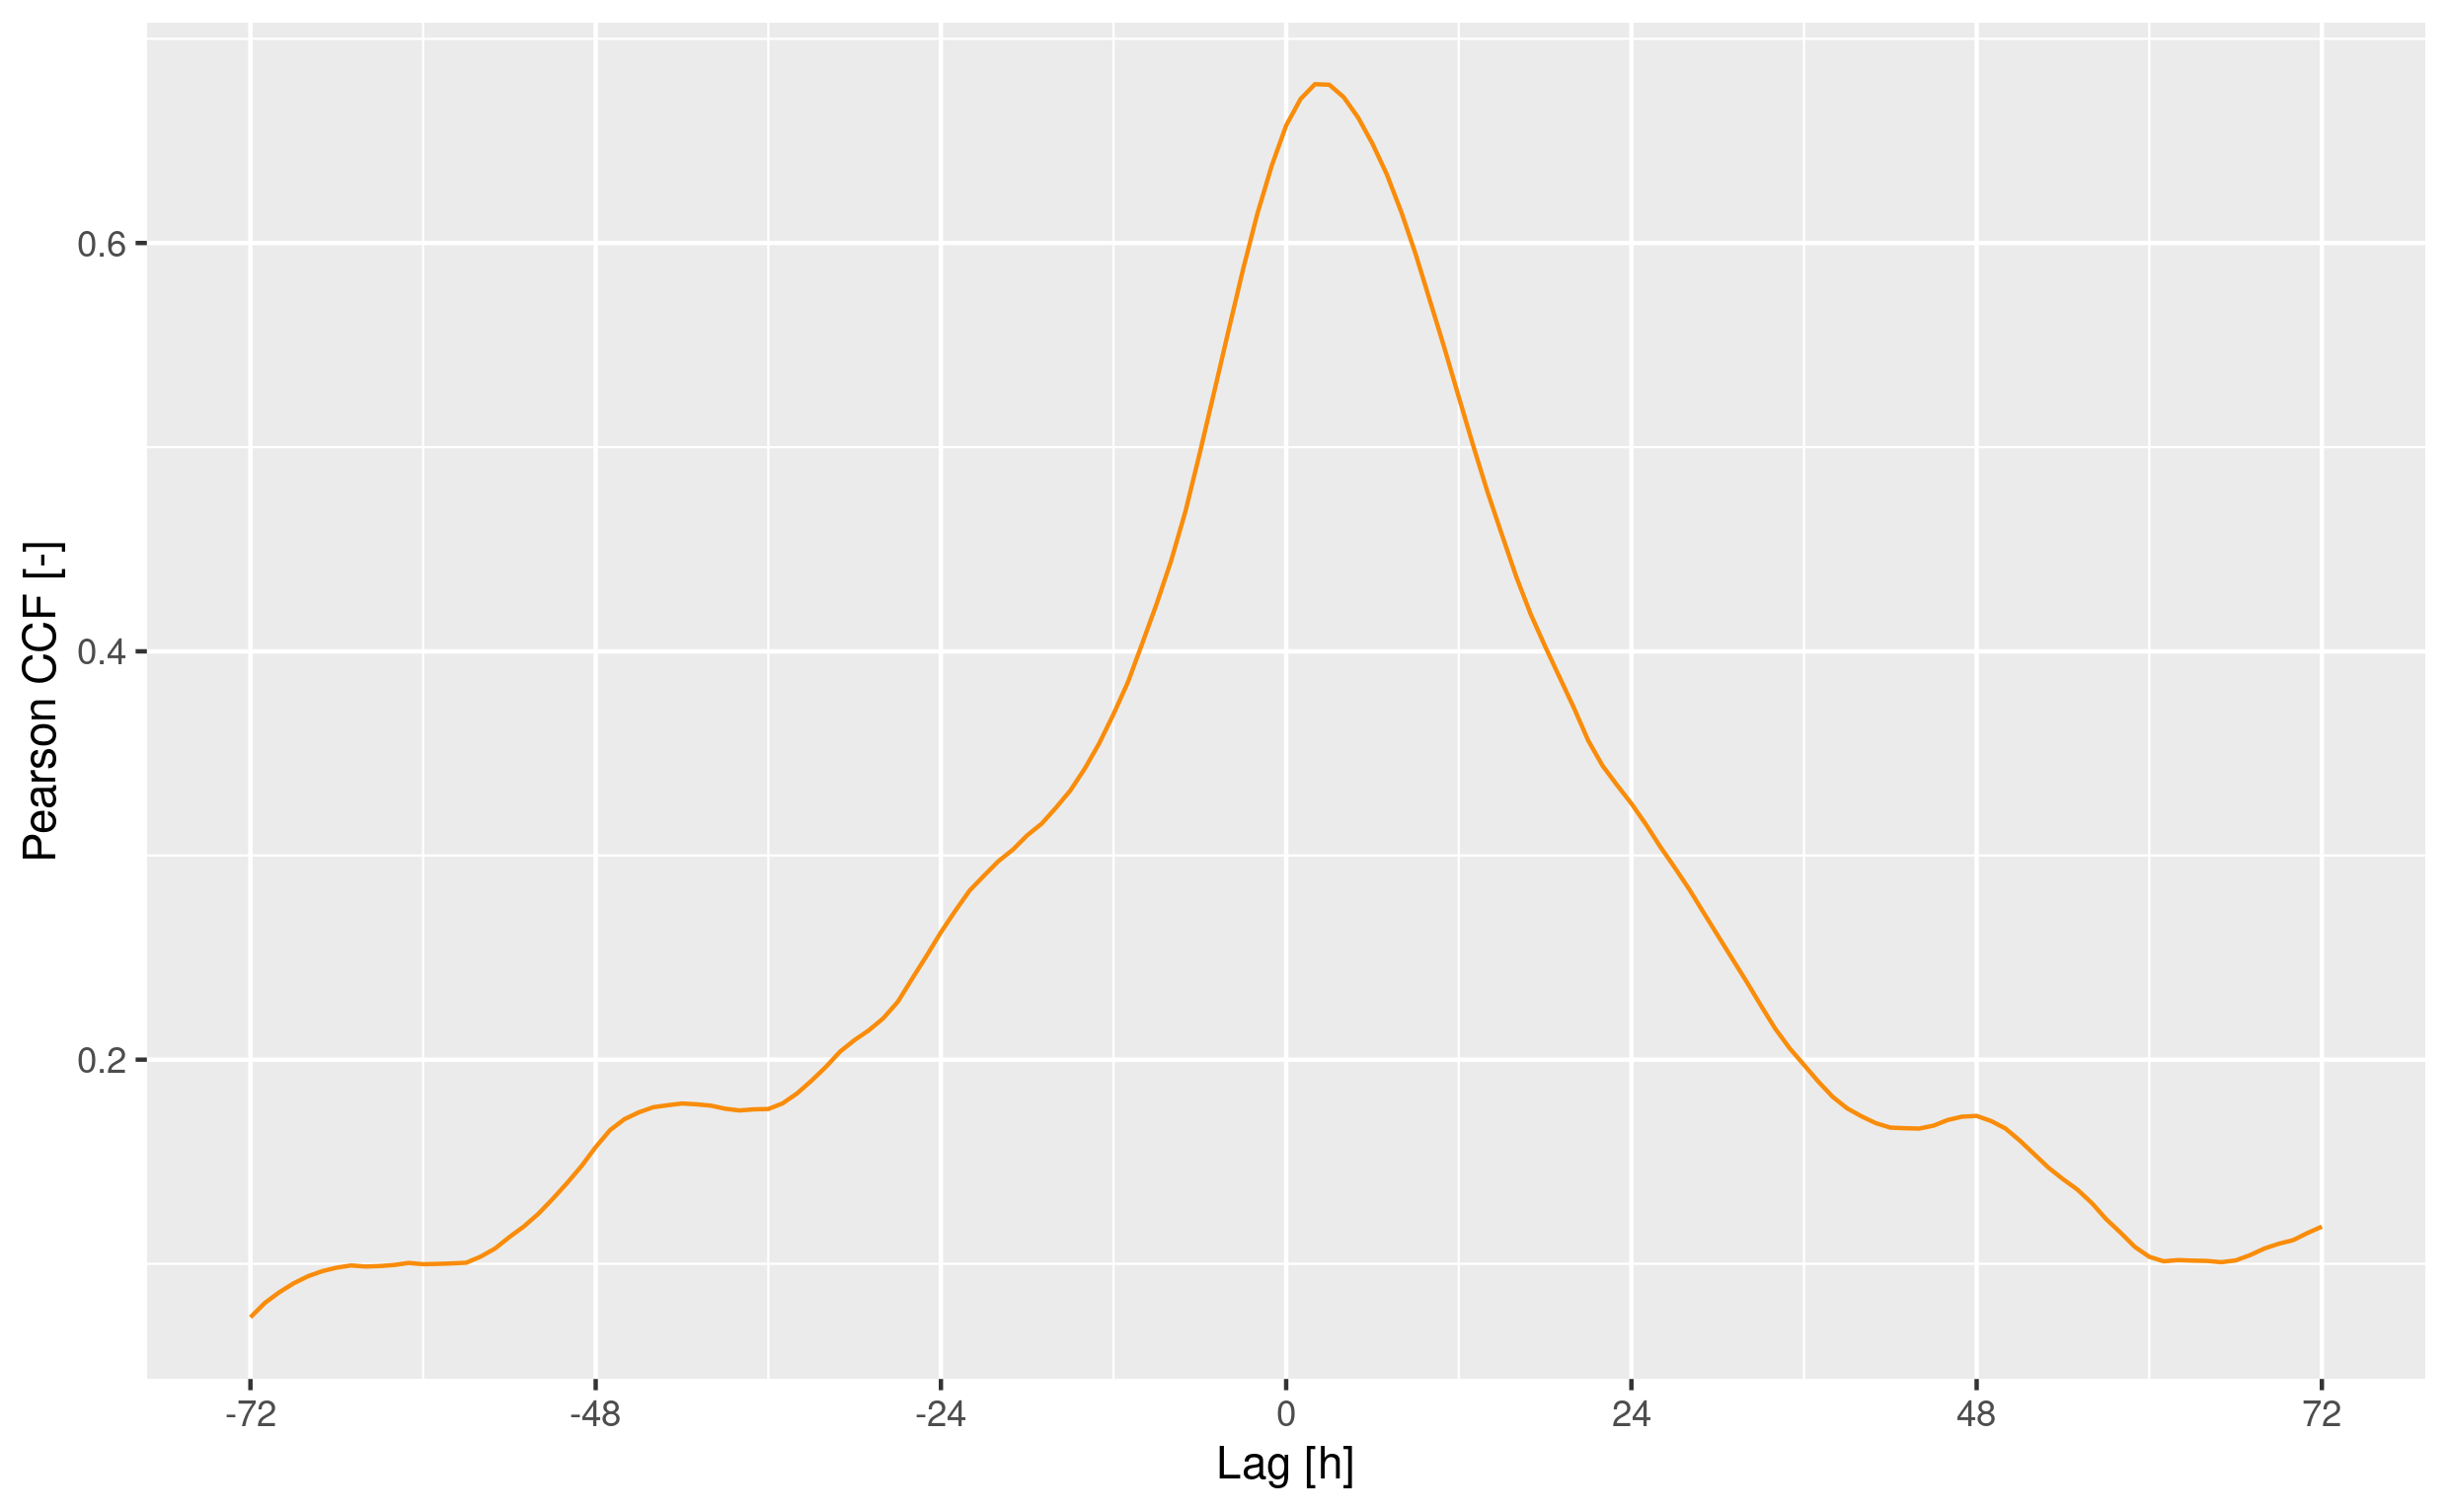
\includegraphics[width=0.8\textwidth]{ccf-sample_20200630_072805}
	\label{fig:ccf}
\end{figure}

\begin{figure}[H]%
	\centering
    \caption{Superposition of cross-correlograms for all $nCR(296, 2)$ pairs of districts.}
    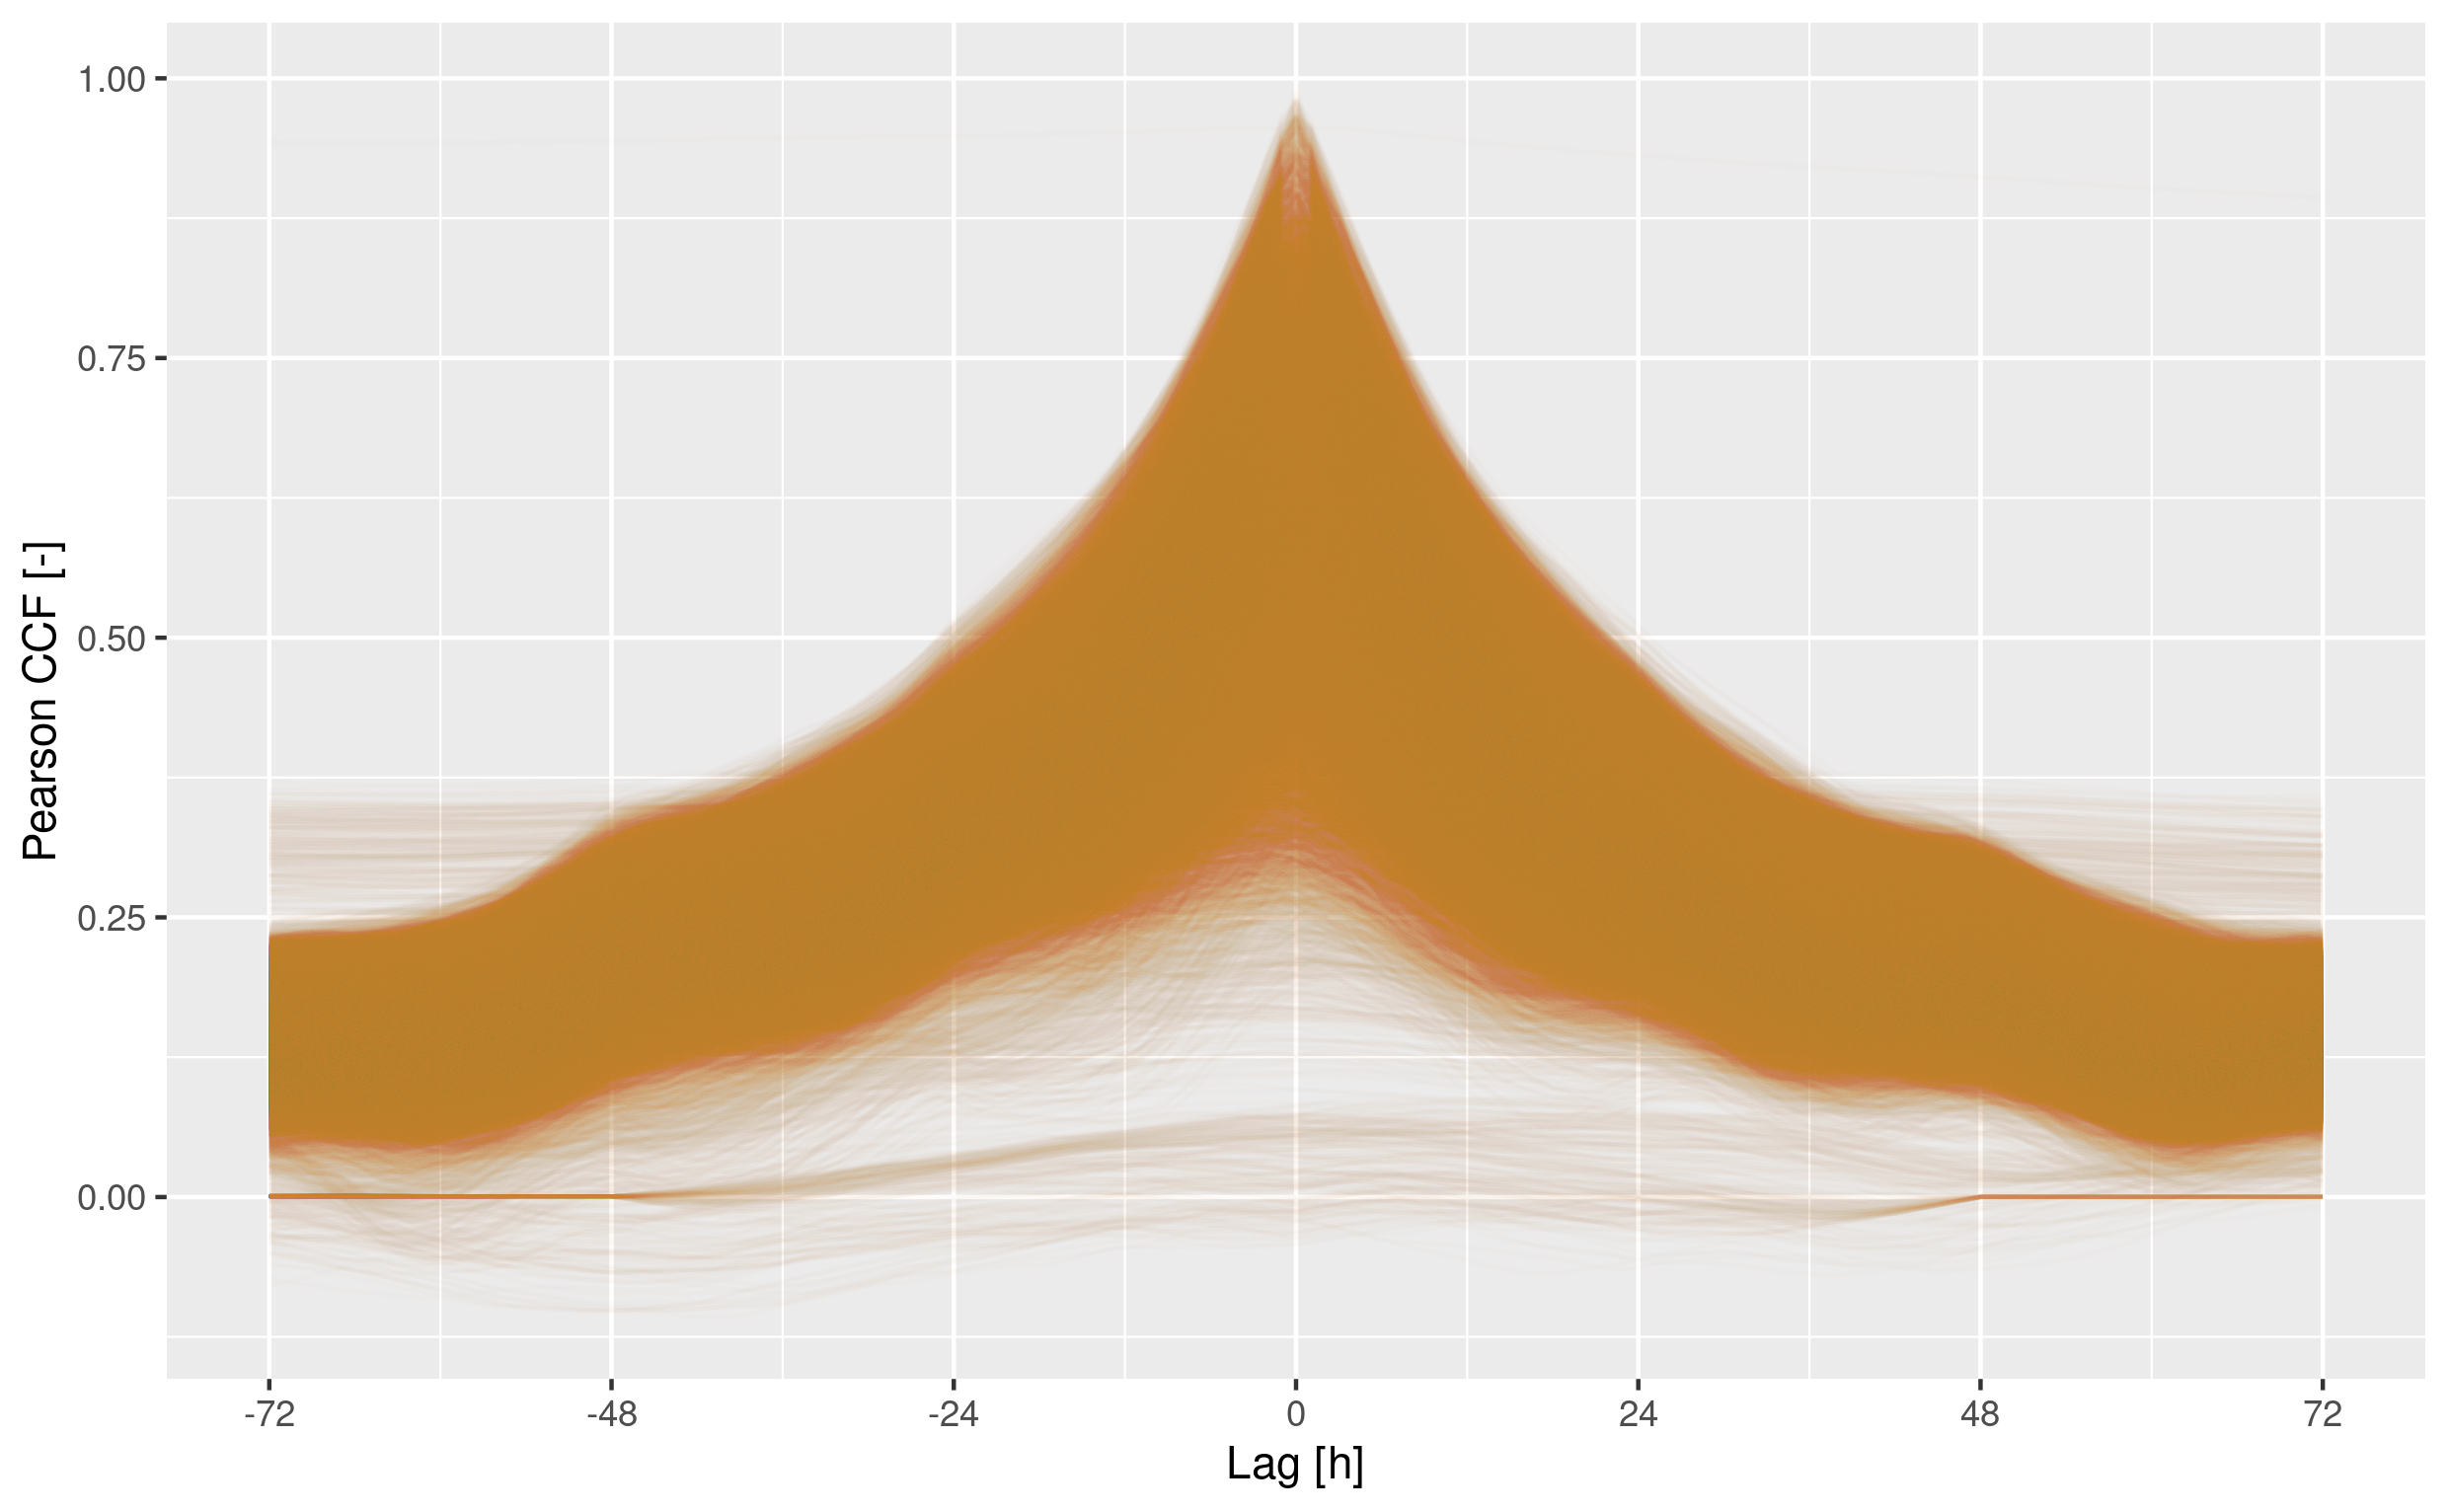
\includegraphics[width=0.8\textwidth]{ccf-all_fav}
	\label{fig:ccf_all}
\end{figure}


\section{Consequences for the data pipeline design}\label{sec:eda_conclusions}

In general, the EDA was important to verify that spatio-temporal dependencies are significant in the use case at hand.
Below, we summarize the main consequences this analysis had to our design decisions.

\vspace{1em}
\noindent
\textbf{Preprocessing.} Handling missing data is not necessary, but scaling the time series e.g. into capacity factors is expected to heavily influence model performances. Weibull-distributed time series might require non-linear scaling.

\vspace{1em}
\noindent
\textbf{Modeling.} Aggregating time series to time resolutions coarser than 12 hours might diminish correlations between them, thus potentially limiting the potential accuracy gains in using spatio-temporal approaches.

\vspace{1em}
\noindent
\textbf{Key modeling assumptions.} In this work, we assume negligible the effects of (a) curtailments, (b) maintenance of individual units, (c) decommissioning of individual units, (d) sudden increases in capacity factor due to technological advances.
